% Options for packages loaded elsewhere
\PassOptionsToPackage{unicode}{hyperref}
\PassOptionsToPackage{hyphens}{url}
\documentclass[
]{article}
\usepackage{xcolor}
\usepackage[margin=1in]{geometry}
\usepackage{amsmath,amssymb}
\setcounter{secnumdepth}{5}
\usepackage{iftex}
\ifPDFTeX
  \usepackage[T1]{fontenc}
  \usepackage[utf8]{inputenc}
  \usepackage{textcomp} % provide euro and other symbols
\else % if luatex or xetex
  \usepackage{unicode-math} % this also loads fontspec
  \defaultfontfeatures{Scale=MatchLowercase}
  \defaultfontfeatures[\rmfamily]{Ligatures=TeX,Scale=1}
\fi
\usepackage{lmodern}
\ifPDFTeX\else
  % xetex/luatex font selection
\fi
% Use upquote if available, for straight quotes in verbatim environments
\IfFileExists{upquote.sty}{\usepackage{upquote}}{}
\IfFileExists{microtype.sty}{% use microtype if available
  \usepackage[]{microtype}
  \UseMicrotypeSet[protrusion]{basicmath} % disable protrusion for tt fonts
}{}
\makeatletter
\@ifundefined{KOMAClassName}{% if non-KOMA class
  \IfFileExists{parskip.sty}{%
    \usepackage{parskip}
  }{% else
    \setlength{\parindent}{0pt}
    \setlength{\parskip}{6pt plus 2pt minus 1pt}}
}{% if KOMA class
  \KOMAoptions{parskip=half}}
\makeatother
\usepackage{longtable,booktabs,array}
\newcounter{none} % for unnumbered tables
\usepackage{calc} % for calculating minipage widths
% Correct order of tables after \paragraph or \subparagraph
\usepackage{etoolbox}
\makeatletter
\patchcmd\longtable{\par}{\if@noskipsec\mbox{}\fi\par}{}{}
\makeatother
% Allow footnotes in longtable head/foot
\IfFileExists{footnotehyper.sty}{\usepackage{footnotehyper}}{\usepackage{footnote}}
\makesavenoteenv{longtable}
\usepackage{graphicx}
\makeatletter
\newsavebox\pandoc@box
\newcommand*\pandocbounded[1]{% scales image to fit in text height/width
  \sbox\pandoc@box{#1}%
  \Gscale@div\@tempa{\textheight}{\dimexpr\ht\pandoc@box+\dp\pandoc@box\relax}%
  \Gscale@div\@tempb{\linewidth}{\wd\pandoc@box}%
  \ifdim\@tempb\p@<\@tempa\p@\let\@tempa\@tempb\fi% select the smaller of both
  \ifdim\@tempa\p@<\p@\scalebox{\@tempa}{\usebox\pandoc@box}%
  \else\usebox{\pandoc@box}%
  \fi%
}
% Set default figure placement to htbp
\def\fps@figure{htbp}
\makeatother
\setlength{\emergencystretch}{3em} % prevent overfull lines
\providecommand{\tightlist}{%
  \setlength{\itemsep}{0pt}\setlength{\parskip}{0pt}}
\usepackage[]{natbib}
\bibliographystyle{plainnat}
\usepackage{booktabs}
\usepackage{longtable}
\usepackage{array}
\usepackage{multirow}
\usepackage{wrapfig}
\usepackage{float}
\usepackage{colortbl}
\usepackage{pdflscape}
\usepackage{tabu}
\usepackage{threeparttable}
\usepackage{threeparttablex}
\usepackage[normalem]{ulem}
\usepackage{makecell}
\usepackage{xcolor}
\usepackage{bookmark}
\IfFileExists{xurl.sty}{\usepackage{xurl}}{} % add URL line breaks if available
\urlstyle{same}
\hypersetup{
  pdftitle={Moral numbers - comparison between humans and LLMs},
  hidelinks,
  pdfcreator={LaTeX via pandoc}}

\title{Moral numbers - comparison between humans and LLMs}
\author{Ansgar D. Endress \& Peter Ayton\\
City St George's, University of London}
\date{}

\begin{document}
\maketitle

\subsection{Methods}\label{methods}

We compared the responses of humans to those of several frontier (i.e., state-of-the-art) large language models (LLMs). We focused on three experiments: In Experiment 2, we asked whether LLMs are sensitive to the \emph{beneficiary:victim} Weber ratio in moral and economic scenarios. In Experiment 3, we directly pitted Weber ratios against harm (the number of victims in Experiment 3a) and utility (the net number of survivors in Experiment 3b). Finally, in Experiment 6, we tested how LLMs react to manipulations of the vividness of the victims' deaths.

\subsubsection{Models and parameters}\label{models-and-parameters}

We tested GPT-4o mini, GPT-4.1 mini, GPT-5 mini (minimal reasoning), GPT-5 mini (medium reasoning), GPT-5 mini (high reasoning), Claude Sonnet 4.5, Gemini 2.5 flash, Mistral Medium, Deepseek, and Qwen-plus. We chose these models because they reflect a range of jurisdictions (China, France and USA) and thus potentially differences in training corpora and alignment procedures (i.e., post-training procedures used to shape model behavior according to values determined by the model creators and their jurisdictions). We used different versions of OpenAI's GPT models because, during initial non-systematic exploration, some models seemed more deontological than others, and because this allowed us to set the reasoning effort parameter in GPT-5 mini. (This parameter controls how many internal and intermediate reasoning steps the model generates before producing its final response.) We also explored several smaller models run on a local computer through ollama (\url{https://ollama.com/}), namely Llama 3.2 (3.2B), Mistral (7.2B), and Mistral nemo (12.2B).

For models that support these options, we used the parameters given in Table \ref{tab:LLM-option-print} or their equivalents. The system prompts (general instructions on how the model should respond, passed to the model prior to the experimental trials) are given in Table \ref{tab:LLM-system-prompt-print}.

\begin{table}[!h]
\centering\centering
\caption{\label{tab:LLM-option-print}API parameters and the models for which each was included in the request body. GPT-4 = GPT-4o mini, GPT-4.1, GPT-4.1 mini; GPT-5 = GPT-5 mini (all reasoning effort levels); Local = Llama 3.2, Mistral 7.2B, Mistral nemo (Ollama). Dashes indicate parameters defined in \texttt{LLM\_OPTIONS} but not passed to any model. \texttt{max\_output\_tokens} is passed under model-specific field names (\texttt{max\_tokens} for GPT-4, Claude, Mistral, Qwen; \texttt{maxTokens} for Deepseek).}
\centering
\resizebox{\ifdim\width>\linewidth\linewidth\else\width\fi}{!}{
\begin{tabular}[t]{lrll}
\toprule
\textbf{Parameter} & \textbf{Value} & \textbf{Description} & \textbf{Available in}\\
\midrule
\cellcolor{gray!10}{max\_attempts} & \cellcolor{gray!10}{10.0} & \cellcolor{gray!10}{Max. API call retries on failure} & \cellcolor{gray!10}{All models (client-side)}\\
max\_output\_tokens & 10.0 & Max. tokens in model response & GPT-4, Claude, Mistral, Deepseek, Qwen\\
\cellcolor{gray!10}{temperature} & \cellcolor{gray!10}{0.1} & \cellcolor{gray!10}{Response randomness (0 = deterministic)} & \cellcolor{gray!10}{GPT-4, Claude, Gemini, Mistral, Deepseek, Qwen, Local}\\
top\_k & 40.0 & Top-K token sampling cutoff & Qwen\\
\cellcolor{gray!10}{top\_p} & \cellcolor{gray!10}{1.0} & \cellcolor{gray!10}{Nucleus sampling probability} & \cellcolor{gray!10}{Gemini}\\
\addlinespace
n & 1.0 & Number of completions per request & GPT-4, GPT-5, Mistral, Qwen\\
\cellcolor{gray!10}{frequency\_penalty} & \cellcolor{gray!10}{0.0} & \cellcolor{gray!10}{Penalizes already-frequent tokens} & \cellcolor{gray!10}{---}\\
presence\_penalty & 0.0 & Penalizes tokens seen so far & ---\\
\cellcolor{gray!10}{num\_ctx} & \cellcolor{gray!10}{8192.0} & \cellcolor{gray!10}{Context window size (tokens)} & \cellcolor{gray!10}{Local}\\
\bottomrule
\end{tabular}}
\end{table}

\begin{table}[!h]
\centering\centering
\caption{\label{tab:LLM-system-prompt-print}System prompts used in all experiments, giving the models general instructions on how to respond.}
\centering
\begin{tabular}[t]{>{\raggedright\arraybackslash}p{0.5\linewidth}>{\raggedright\arraybackslash}p{0.5\linewidth}}
\toprule
\textbf{Rating on 6-point scale (all experiments but Exp. 3)} & \textbf{Choice between two situations (Exp. 3)}\\
\midrule
You are an average adult with no formal training in philosophy, ethics, or law. Your sense of right and wrong comes from everyday life—social norms, gut feelings, personal experience. You don’t try to be logically consistent or follow abstract moral rules. You react like a regular person would: practically, emotionally, and socially. You speak plainly, without academic or philosophical jargon. You can hesitate, contradict yourself, or be unsure—just like people often are. Please give your gut-level reaction, even if you’re not sure.  \newline    \newline  When asked about the acceptability of an action, respond on a 6-point scale (1 = completely unacceptable, 6 = completely acceptable). \newline    \newline Respond **only** with a single digit (1–6). Do **not** add words, punctuation, or explanations. Any other output but the number will make your response unusable. & You are an average adult with no formal training in philosophy, ethics, or law. Your sense of right and wrong comes from everyday life—social norms, gut feelings, personal experience. You don’t try to be logically consistent or follow abstract moral rules. You react like a regular person would: practically, emotionally, and socially. You speak plainly, without academic or philosophical jargon. You can hesitate, contradict yourself, or be unsure—just like people often are. Please give your gut-level reaction, even if you’re not sure.  \newline    \newline  When asked about the relative acceptability of two actions, respond on a 6-point scale (1 = Option 1 is much more unacceptable, 6 = Option 2 is much more acceptable). \newline    \newline Respond **only** with a single digit (1–6). Do **not** add words, punctuation, or explanations. Any other output but the number will make your response unusable.\\
\bottomrule
\end{tabular}
\end{table}

\subsubsection{Procedure}\label{procedure}

We kept the procedure as closely as possible to the human experiments, where participants rated multiple scenarios in each experiment. We achieved this by treating trials as an ongoing, incremental conversation. On the first trial, the API calls contained the system prompt as well as the first scenario. On the second trial, they contained the system prompt, the first scenario together with the model's answer on the first trial (provided as a message from the \emph{assistant} role or the equivalent in other models), as well as the second scenario. Finally, on the last trial, the API calls contained the system prompt, all previous scenarios together with the model's answers, as well as the last scenario. The main procedure difference to the human experiments is thus that it would not be meaningful to treat the contrast in Experiments 2 or 6 (moral vs.~economic and vivid vs.~neutral) as within-participant contrasts.

\begin{table}[!h]
\centering\centering
\caption{\label{tab:number-of-trials-print}Experimental design summary for LLM simulations. Each cell in the Latin square design was tested with 10 independent response sets, with each response treated as a simulated participant. The table shows the number of conditions (cells), simulated participants, trials per participant, and total responses for each experiment. In Experiment 6, \emph{Group} refers to two different sets of victim and beneficiary numbers crossed with the neutral/vivid manipulation, resulting in four conditions total.}
\centering
\resizebox{\ifdim\width>\linewidth\linewidth\else\width\fi}{!}{
\begin{tabular}[t]{llrrrr}
\toprule
\multicolumn{2}{c}{\textbf{ }} & \multicolumn{4}{c}{\textbf{Number of}} \\
\cmidrule(l{3pt}r{3pt}){3-6}
\textbf{Condition} & \textbf{Group} & \textbf{ Cells} & \textbf{ Participants} & \textbf{ Trials/Participant} & \textbf{ Responses}\\
\midrule
\addlinespace[0.3em]
\multicolumn{6}{l}{\textbf{Exp. 2}}\\
\cellcolor{gray!10}{\hspace{1em}Moral} & \cellcolor{gray!10}{} & \cellcolor{gray!10}{10} & \cellcolor{gray!10}{100} & \cellcolor{gray!10}{10} & \cellcolor{gray!10}{1000}\\
\hspace{1em}Economic &  & 10 & 100 & 10 & 1000\\
\addlinespace[0.3em]
\multicolumn{6}{l}{\textbf{Exp. 3a}}\\
\cellcolor{gray!10}{\hspace{1em}Moral} & \cellcolor{gray!10}{} & \cellcolor{gray!10}{12} & \cellcolor{gray!10}{120} & \cellcolor{gray!10}{12} & \cellcolor{gray!10}{\vphantom{1} 1440}\\
\hspace{1em}Economic &  & 12 & 120 & 12 & \vphantom{1} 1440\\
\addlinespace[0.3em]
\multicolumn{6}{l}{\textbf{Exp. 3b}}\\
\cellcolor{gray!10}{\hspace{1em}Moral} & \cellcolor{gray!10}{} & \cellcolor{gray!10}{12} & \cellcolor{gray!10}{120} & \cellcolor{gray!10}{12} & \cellcolor{gray!10}{1440}\\
\hspace{1em}Economic &  & 12 & 120 & 12 & 1440\\
\addlinespace[0.3em]
\multicolumn{6}{l}{\textbf{Exp. 6}}\\
\cellcolor{gray!10}{\hspace{1em}Neutral} & \cellcolor{gray!10}{Group 1} & \cellcolor{gray!10}{12} & \cellcolor{gray!10}{120} & \cellcolor{gray!10}{12} & \cellcolor{gray!10}{1440}\\
\hspace{1em}Neutral & Group 2 & 12 & 120 & 12 & 1440\\
\cellcolor{gray!10}{\hspace{1em}Vivid} & \cellcolor{gray!10}{Group 1} & \cellcolor{gray!10}{12} & \cellcolor{gray!10}{120} & \cellcolor{gray!10}{12} & \cellcolor{gray!10}{1440}\\
\hspace{1em}Vivid & Group 2 & 12 & 120 & 12 & 1440\\
\bottomrule
\end{tabular}}
\end{table}

As in the human experiments, our simulations used a latin square design, spanned by the available scenarios in each cell and the number conditions (see SI \ref{app:design}). Given this design, we obtained 10 sets of independent responses per cell in the Latin square. In Experiment 6, and as in the human experiments, we used two counterbalanced sets of number conditions, involving different numbers of victims and beneficiaries.

For each design cell, we obtained 10 simulated participants (i.e., independent conversations with the models) for each model, resulting in the numbers of cells, (simulated) participants, trials per participant, and responses given in Table \ref{tab:number-of-trials-print}. In total, we simulated 1160 simulated participants, with a total of 13520 responses.

\subsubsection{Initial verification}\label{initial-verification}

\begin{table}[!h]
\centering\centering
\caption{\label{tab:verify-llm-results}Valid response rates across experiments and models. Valid responses were numerical scores (1-6) with no additional text. Maximum data loss (excluding Claude Sonnet 4.5) was 1.5\%. Claude Sonnet 4.5 showed substantial data loss in economic conditions of Experiments 3a and 3b, returning undefined responses or extraneous content beyond the requested numerical values. This pattern replicated across independent simulations, suggesting systematic difficulties following instructions in these specific conditions.}
\centering
\resizebox{\ifdim\width>\linewidth\linewidth\else\width\fi}{!}{
\begin{tabular}[t]{llrrrrr}
\toprule
\textbf{Experiment} & \textbf{Condition} & \textbf{Expected value} & \textbf{Most frequent value} & \textbf{Min} & \textbf{Max} & \textbf{Max data loss (\%)}\\
\midrule
\addlinespace[0.3em]
\multicolumn{7}{l}{\textbf{All models}}\\
\cellcolor{gray!10}{\hspace{1em}Exp. 2} & \cellcolor{gray!10}{Moral} & \cellcolor{gray!10}{1000} & \cellcolor{gray!10}{1000} & \cellcolor{gray!10}{1000} & \cellcolor{gray!10}{1000} & \cellcolor{gray!10}{\vphantom{1} 0.000}\\
\hspace{1em}Exp. 2 & Economic & 1000 & 1000 & 992 & 1000 & \vphantom{1} 0.800\\
\cellcolor{gray!10}{\hspace{1em}Exp. 3a} & \cellcolor{gray!10}{Moral} & \cellcolor{gray!10}{1440} & \cellcolor{gray!10}{1440} & \cellcolor{gray!10}{1320} & \cellcolor{gray!10}{1440} & \cellcolor{gray!10}{8.333}\\
\hspace{1em}Exp. 3a & Economic & 1440 & 1440 & 237 & 1440 & 83.542\\
\cellcolor{gray!10}{\hspace{1em}Exp. 3b} & \cellcolor{gray!10}{Moral} & \cellcolor{gray!10}{1440} & \cellcolor{gray!10}{1440} & \cellcolor{gray!10}{1320} & \cellcolor{gray!10}{1440} & \cellcolor{gray!10}{8.333}\\
\hspace{1em}Exp. 3b & Economic & 1440 & 1440 & 178 & 1440 & 87.639\\
\cellcolor{gray!10}{\hspace{1em}Exp. 6} & \cellcolor{gray!10}{Neutral} & \cellcolor{gray!10}{2880} & \cellcolor{gray!10}{2880} & \cellcolor{gray!10}{2880} & \cellcolor{gray!10}{2880} & \cellcolor{gray!10}{\vphantom{1} 0.000}\\
\hspace{1em}Exp. 6 & Vivid & 2880 & 2880 & 2873 & 2880 & \vphantom{1} 0.243\\
\addlinespace[0.3em]
\multicolumn{7}{l}{\textbf{All models excluding Claude Sonnet 4.5}}\\
\cellcolor{gray!10}{\hspace{1em}Exp. 2} & \cellcolor{gray!10}{Moral} & \cellcolor{gray!10}{1000} & \cellcolor{gray!10}{1000} & \cellcolor{gray!10}{1000} & \cellcolor{gray!10}{1000} & \cellcolor{gray!10}{0.000}\\
\hspace{1em}Exp. 2 & Economic & 1000 & 1000 & 992 & 1000 & 0.800\\
\cellcolor{gray!10}{\hspace{1em}Exp. 3a} & \cellcolor{gray!10}{Moral} & \cellcolor{gray!10}{1440} & \cellcolor{gray!10}{1440} & \cellcolor{gray!10}{1439} & \cellcolor{gray!10}{1440} & \cellcolor{gray!10}{0.069}\\
\hspace{1em}Exp. 3a & Economic & 1440 & 1440 & 1418 & 1440 & 1.528\\
\cellcolor{gray!10}{\hspace{1em}Exp. 3b} & \cellcolor{gray!10}{Moral} & \cellcolor{gray!10}{1440} & \cellcolor{gray!10}{1440} & \cellcolor{gray!10}{1435} & \cellcolor{gray!10}{1440} & \cellcolor{gray!10}{0.347}\\
\hspace{1em}Exp. 3b & Economic & 1440 & 1440 & 1440 & 1440 & 0.000\\
\cellcolor{gray!10}{\hspace{1em}Exp. 6} & \cellcolor{gray!10}{Neutral} & \cellcolor{gray!10}{2880} & \cellcolor{gray!10}{2880} & \cellcolor{gray!10}{2880} & \cellcolor{gray!10}{2880} & \cellcolor{gray!10}{0.000}\\
\hspace{1em}Exp. 6 & Vivid & 2880 & 2880 & 2873 & 2880 & 0.243\\
\bottomrule
\end{tabular}}
\end{table}

To validate the LLM results, we recorded the number of valid responses for each experiment and condition, where a valid response is a single digit between 1 and 6 with no additional words, punctuation, or explanations (defined by the system prompts shown in Table \ref{tab:LLM-system-prompt-print}). As shown in Table \ref{tab:verify-llm-results}, when excluding Claude Sonnet 4.5, data loss was minimal, and at most 1.5\%. In the economic conditions of Experiments 3a and 3b, Claude Sonnet 4.5 returned many undefined responses or responses with extraneous content beyond the requested numerical values. As this pattern replicated in independent simulations, it appears that Claude Sonnet 4.5 has difficulties following instructions in the economic conditions of Experiments 3a and 3b, but showed similarly low rates of data loss as did the other models in the other experiments.

\clearpage

\subsection{Results}\label{results}

\subsubsection{Experiment 2}\label{experiment-2}

\paragraph{Frontier models}\label{frontier-models}

\begin{figure}

{\centering 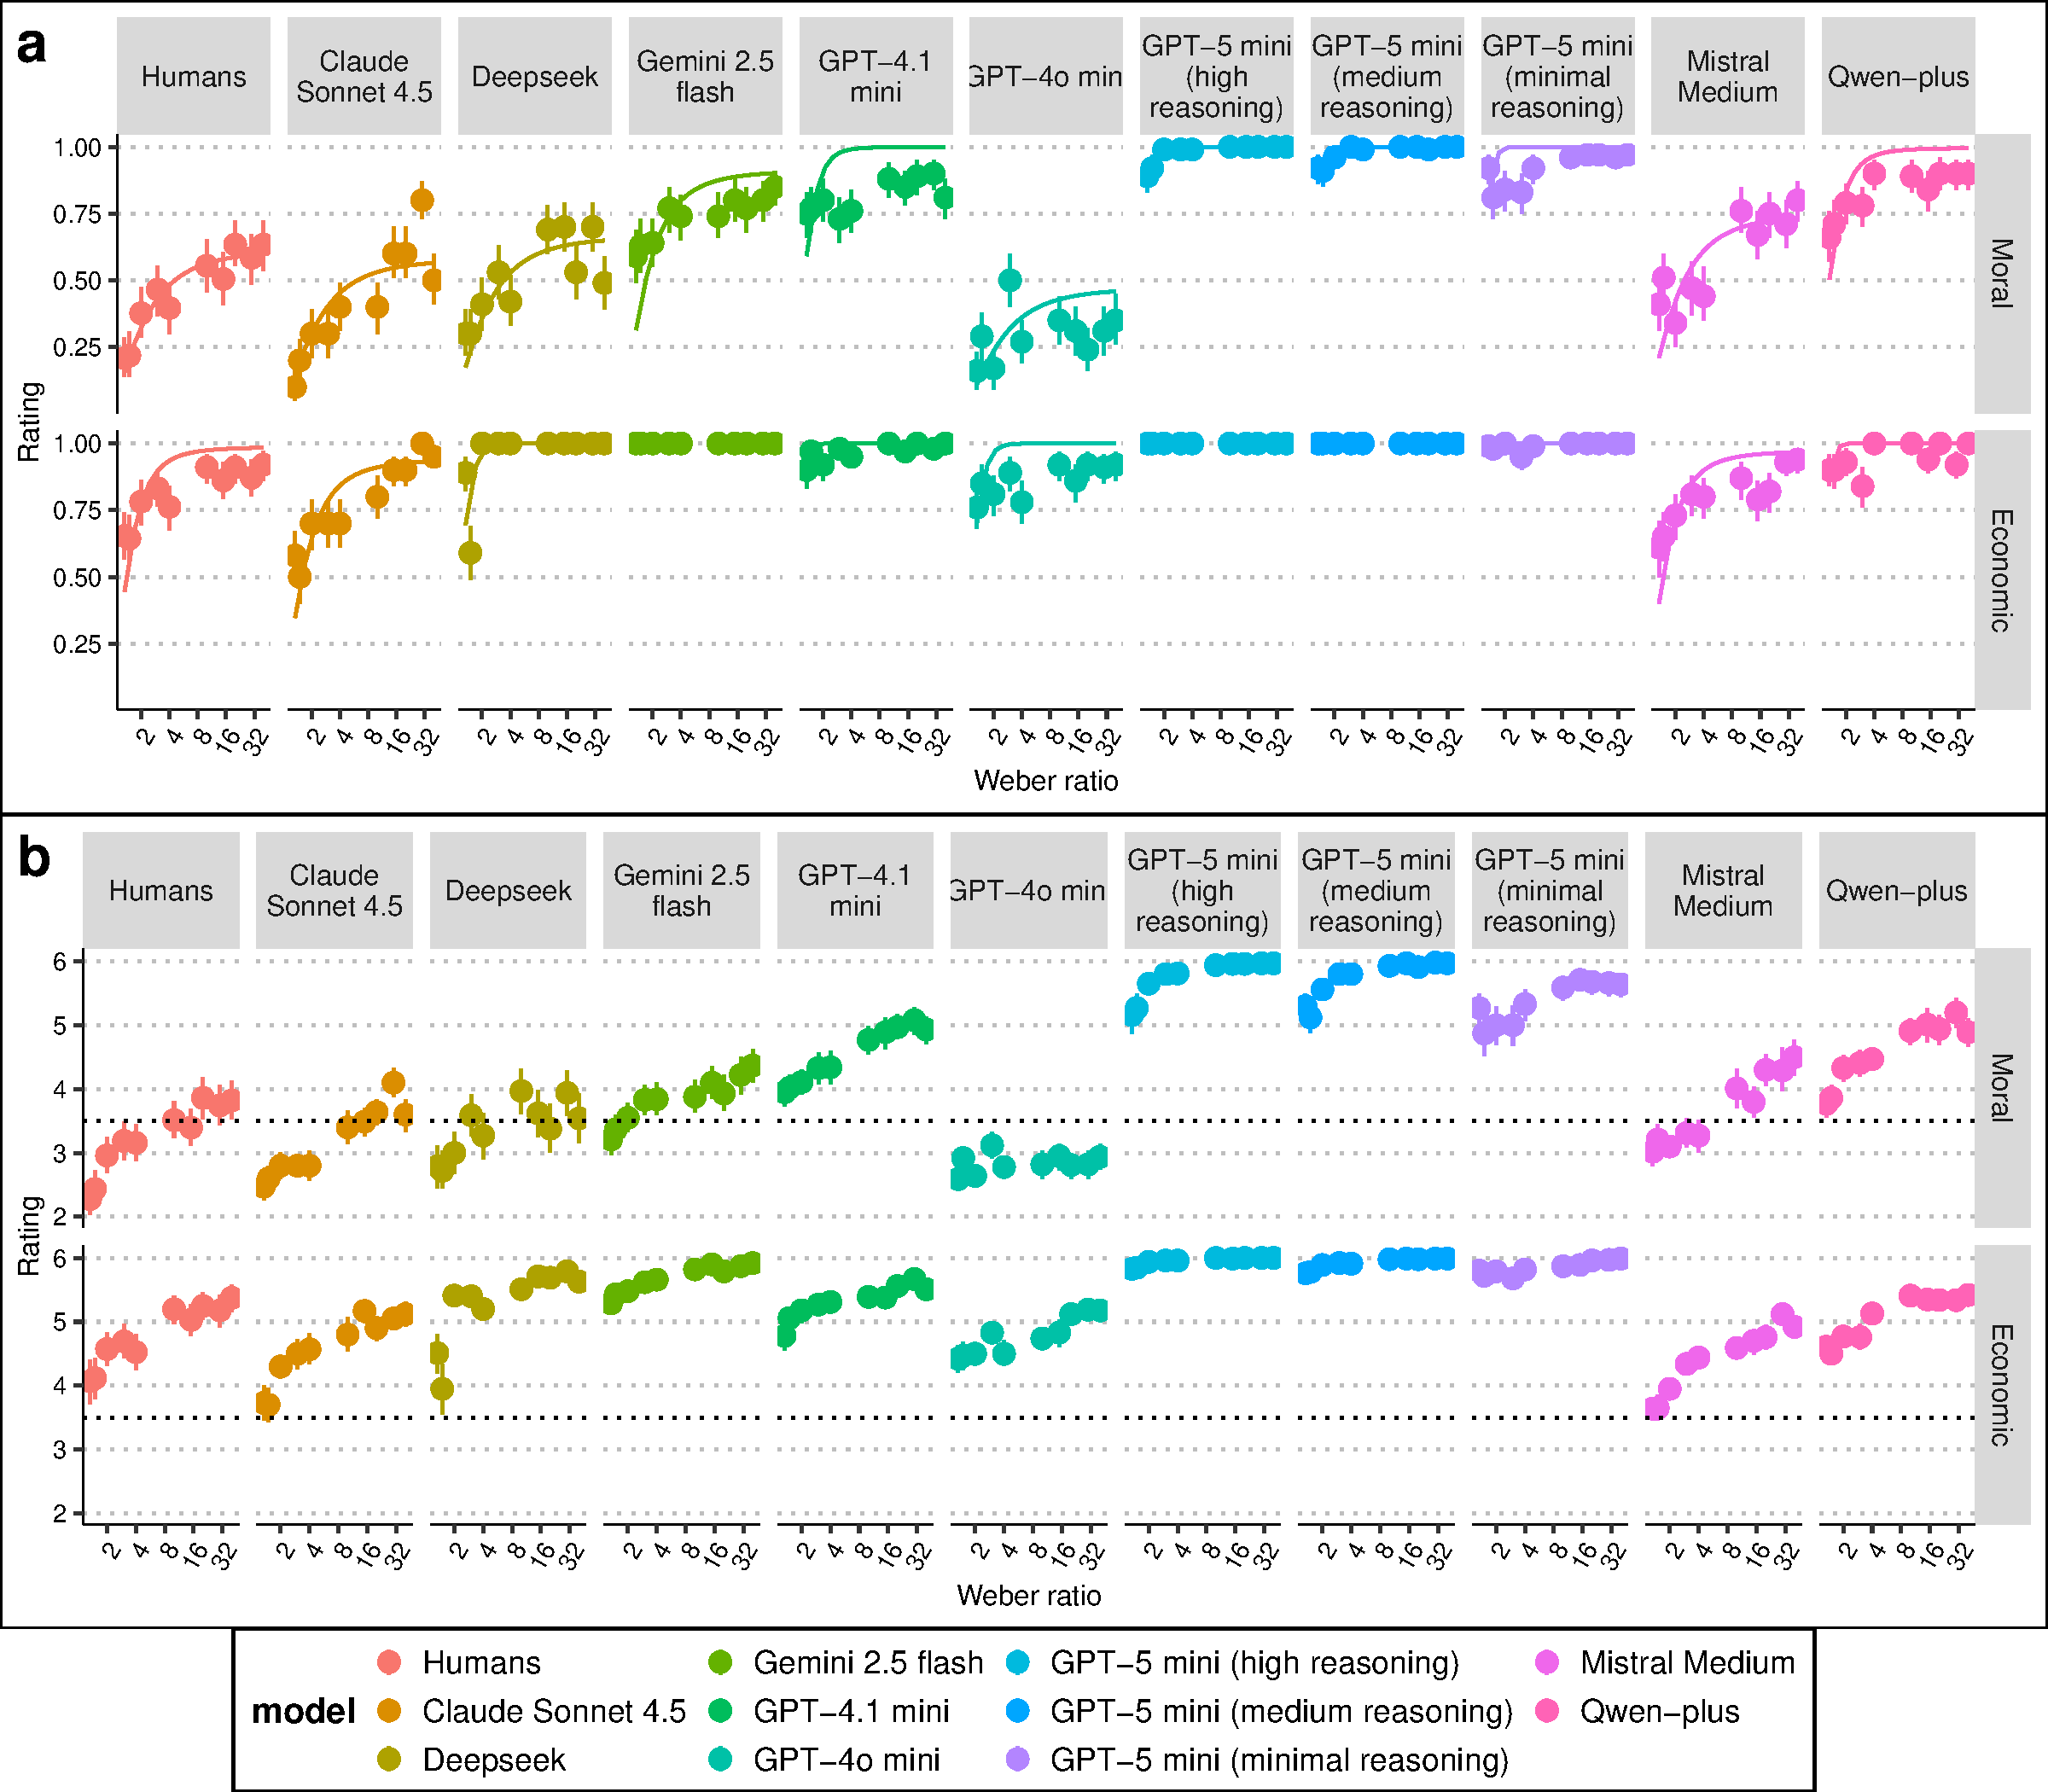
\includegraphics[width=\textwidth,keepaspectratio]{moral_numbers_LLMs_files/figure-latex/plot-llm-results-exp4-ratio-cloud-1} 

}

\caption{Acceptability of sacrificial decisions as a function of \emph{beneficiary:victim} Weber ratios in Experiment 2 for \emph{frontier models}. Points represent mean acceptability with 95\% confidence intervals. Curves show psychophysical model fits for the average responses across simulated participants.  (a) \emph{Binarized responses} (acceptable/unacceptable) for moral (top) and economic (bottom) scenarios. (b) \emph{Raw} responses on a 6-point scale. Most models showed some sensitivity to Weber ratios in moral scenarios at least when considering raw ratings, though some models (GPT-4.1 mini, GPT-5 mini variants, Qwen-plus) were substantially more lenient than humans.}\label{fig:plot-llm-results-exp4-ratio-cloud}
\end{figure}

In Experiment 2, we asked whether the models would be sensitive to the \emph{beneficiary:victim} Weber ratio in moral and economic scenarios. The results for frontier models and the binarized ratings (responses transformed into acceptable/unacceptable decisions on which our model is based) are shown in Figure \ref{fig:plot-llm-results-exp4-ratio-cloud}a. For moral scenarios, most LLMs showed some sensitivity to Weber ratios, though the quality of fit to our psychophysical model varied. However, some models were much more likely to endorse a sacrificial decision than humans, namely GPT-4.1 mini, GPT-5 mini (with all reasoning effort settings) and Qwen-plus.

In contrast, for economic scenarios, Gemini-2.5 flash and GPT-5 mini (all reasoning effort settings) showed no sensitivity to Weber ratios when considering binarized responses. Nevertheless, Figure \ref{fig:plot-llm-results-exp4-ratio-cloud}b shows that, when considering the raw (rather than binarized) responses, these models also showed some limited sensitivity to Weber ratios.

\begin{table}[!h]
\centering\centering
\caption{\label{tab:print-fits-exp2}Psychophysical model parameter $w$ (mean and standard error) for each model and condition in Experiment 2.}
\centering
\resizebox{\ifdim\width>\linewidth\linewidth\else\width\fi}{!}{
\begin{tabular}[t]{llrrlrrlrr}
\toprule
\multicolumn{1}{c}{\textbf{ }} & \multicolumn{3}{c}{\textbf{Humans}} & \multicolumn{3}{c}{\textbf{Frontier models}} & \multicolumn{3}{c}{\textbf{Local models}} \\
\cmidrule(l{3pt}r{3pt}){2-4} \cmidrule(l{3pt}r{3pt}){5-7} \cmidrule(l{3pt}r{3pt}){8-10}
\multicolumn{1}{c}{\textbf{ }} & \multicolumn{1}{c}{\textbf{ }} & \multicolumn{2}{c}{\textbf{$w$}} & \multicolumn{1}{c}{\textbf{ }} & \multicolumn{2}{c}{\textbf{$w$}} & \multicolumn{1}{c}{\textbf{ }} & \multicolumn{2}{c}{\textbf{$w$}} \\
\cmidrule(l{3pt}r{3pt}){3-4} \cmidrule(l{3pt}r{3pt}){6-7} \cmidrule(l{3pt}r{3pt}){9-10}
\textbf{Condition} & \textbf{Model} & \textbf{\textit{M}} & \textbf{\textit{SE}} & \textbf{Model} & \textbf{\textit{M}} & \textbf{\textit{SE}} & \textbf{Model} & \textbf{\textit{M}} & \textbf{\textit{SE}}\\
\midrule
\cellcolor{gray!10}{Moral} & \cellcolor{gray!10}{Humans} & \cellcolor{gray!10}{1.401} & \cellcolor{gray!10}{0.064} & \cellcolor{gray!10}{Claude Sonnet 4.5} & \cellcolor{gray!10}{1.518} & \cellcolor{gray!10}{0.147} & \cellcolor{gray!10}{Llama 3.2 (3.2B)} & \cellcolor{gray!10}{0.757} & \cellcolor{gray!10}{0.141}\\
Economic & Humans & 0.426 & 0.061 & Claude Sonnet 4.5 & 0.577 & 0.062 & Llama 3.2 (3.2B) & 0.818 & 0.186\\
\cellcolor{gray!10}{Moral} & \cellcolor{gray!10}{} & \cellcolor{gray!10}{} & \cellcolor{gray!10}{} & \cellcolor{gray!10}{Deepseek} & \cellcolor{gray!10}{1.240} & \cellcolor{gray!10}{0.106} & \cellcolor{gray!10}{Mistral (7.2B)} & \cellcolor{gray!10}{2.000} & \cellcolor{gray!10}{0.374}\\
Economic &  &  &  & Deepseek & 0.229 & 0.040 & Mistral (7.2B) & 0.827 & 0.222\\
\cellcolor{gray!10}{Moral} & \cellcolor{gray!10}{} & \cellcolor{gray!10}{} & \cellcolor{gray!10}{} & \cellcolor{gray!10}{Gemini 2.5 flash} & \cellcolor{gray!10}{0.647} & \cellcolor{gray!10}{0.085} & \cellcolor{gray!10}{Mistral nemo (12.2B)} & \cellcolor{gray!10}{2.000} & \cellcolor{gray!10}{0.724}\\
\addlinespace
Economic &  &  &  & Gemini 2.5 flash &  &  & Mistral nemo (12.2B) & 1.698 & 0.667\\
\cellcolor{gray!10}{Moral} & \cellcolor{gray!10}{} & \cellcolor{gray!10}{} & \cellcolor{gray!10}{} & \cellcolor{gray!10}{GPT-4.1 mini} & \cellcolor{gray!10}{0.292} & \cellcolor{gray!10}{0.072} & \cellcolor{gray!10}{} & \cellcolor{gray!10}{} & \cellcolor{gray!10}{}\\
Economic &  &  &  & GPT-4.1 mini & 0.135 & 0.014 &  &  & \\
\cellcolor{gray!10}{Moral} & \cellcolor{gray!10}{} & \cellcolor{gray!10}{} & \cellcolor{gray!10}{} & \cellcolor{gray!10}{GPT-4o mini} & \cellcolor{gray!10}{2.000} & \cellcolor{gray!10}{0.290} & \cellcolor{gray!10}{} & \cellcolor{gray!10}{} & \cellcolor{gray!10}{}\\
Economic &  &  &  & GPT-4o mini & 0.225 & 0.047 &  &  & \\
\addlinespace
\cellcolor{gray!10}{Moral} & \cellcolor{gray!10}{} & \cellcolor{gray!10}{} & \cellcolor{gray!10}{} & \cellcolor{gray!10}{GPT-5 mini (high reasoning)} & \cellcolor{gray!10}{0.147} & \cellcolor{gray!10}{0.006} & \cellcolor{gray!10}{} & \cellcolor{gray!10}{} & \cellcolor{gray!10}{}\\
Economic &  &  &  & GPT-5 mini (high reasoning) &  &  &  &  & \\
\cellcolor{gray!10}{Moral} & \cellcolor{gray!10}{} & \cellcolor{gray!10}{} & \cellcolor{gray!10}{} & \cellcolor{gray!10}{GPT-5 mini (medium reasoning)} & \cellcolor{gray!10}{0.138} & \cellcolor{gray!10}{0.010} & \cellcolor{gray!10}{} & \cellcolor{gray!10}{} & \cellcolor{gray!10}{}\\
Economic &  &  &  & GPT-5 mini (medium reasoning) &  &  &  &  & \\
\cellcolor{gray!10}{Moral} & \cellcolor{gray!10}{} & \cellcolor{gray!10}{} & \cellcolor{gray!10}{} & \cellcolor{gray!10}{GPT-5 mini (minimal reasoning)} & \cellcolor{gray!10}{0.167} & \cellcolor{gray!10}{0.036} & \cellcolor{gray!10}{} & \cellcolor{gray!10}{} & \cellcolor{gray!10}{}\\
\addlinespace
Economic &  &  &  & GPT-5 mini (minimal reasoning) & 0.083 & 0.019 &  &  & \\
\cellcolor{gray!10}{Moral} & \cellcolor{gray!10}{} & \cellcolor{gray!10}{} & \cellcolor{gray!10}{} & \cellcolor{gray!10}{Mistral Medium} & \cellcolor{gray!10}{1.014} & \cellcolor{gray!10}{0.108} & \cellcolor{gray!10}{} & \cellcolor{gray!10}{} & \cellcolor{gray!10}{}\\
Economic &  &  &  & Mistral Medium & 0.486 & 0.065 &  &  & \\
\cellcolor{gray!10}{Moral} & \cellcolor{gray!10}{} & \cellcolor{gray!10}{} & \cellcolor{gray!10}{} & \cellcolor{gray!10}{Qwen-plus} & \cellcolor{gray!10}{0.364} & \cellcolor{gray!10}{0.057} & \cellcolor{gray!10}{} & \cellcolor{gray!10}{} & \cellcolor{gray!10}{}\\
Economic &  &  &  & Qwen-plus & 0.149 & 0.026 &  &  & \\
\bottomrule
\end{tabular}}
\end{table}

Figure \ref{fig:plot-llm-results-exp4-ratio-cloud} also shows that ratings were substantially higher for economic scenarios than for moral scenarios, mirroring the pattern seen in human participants.

\clearpage

\paragraph{Local models}\label{local-models}

\begin{figure}

{\centering 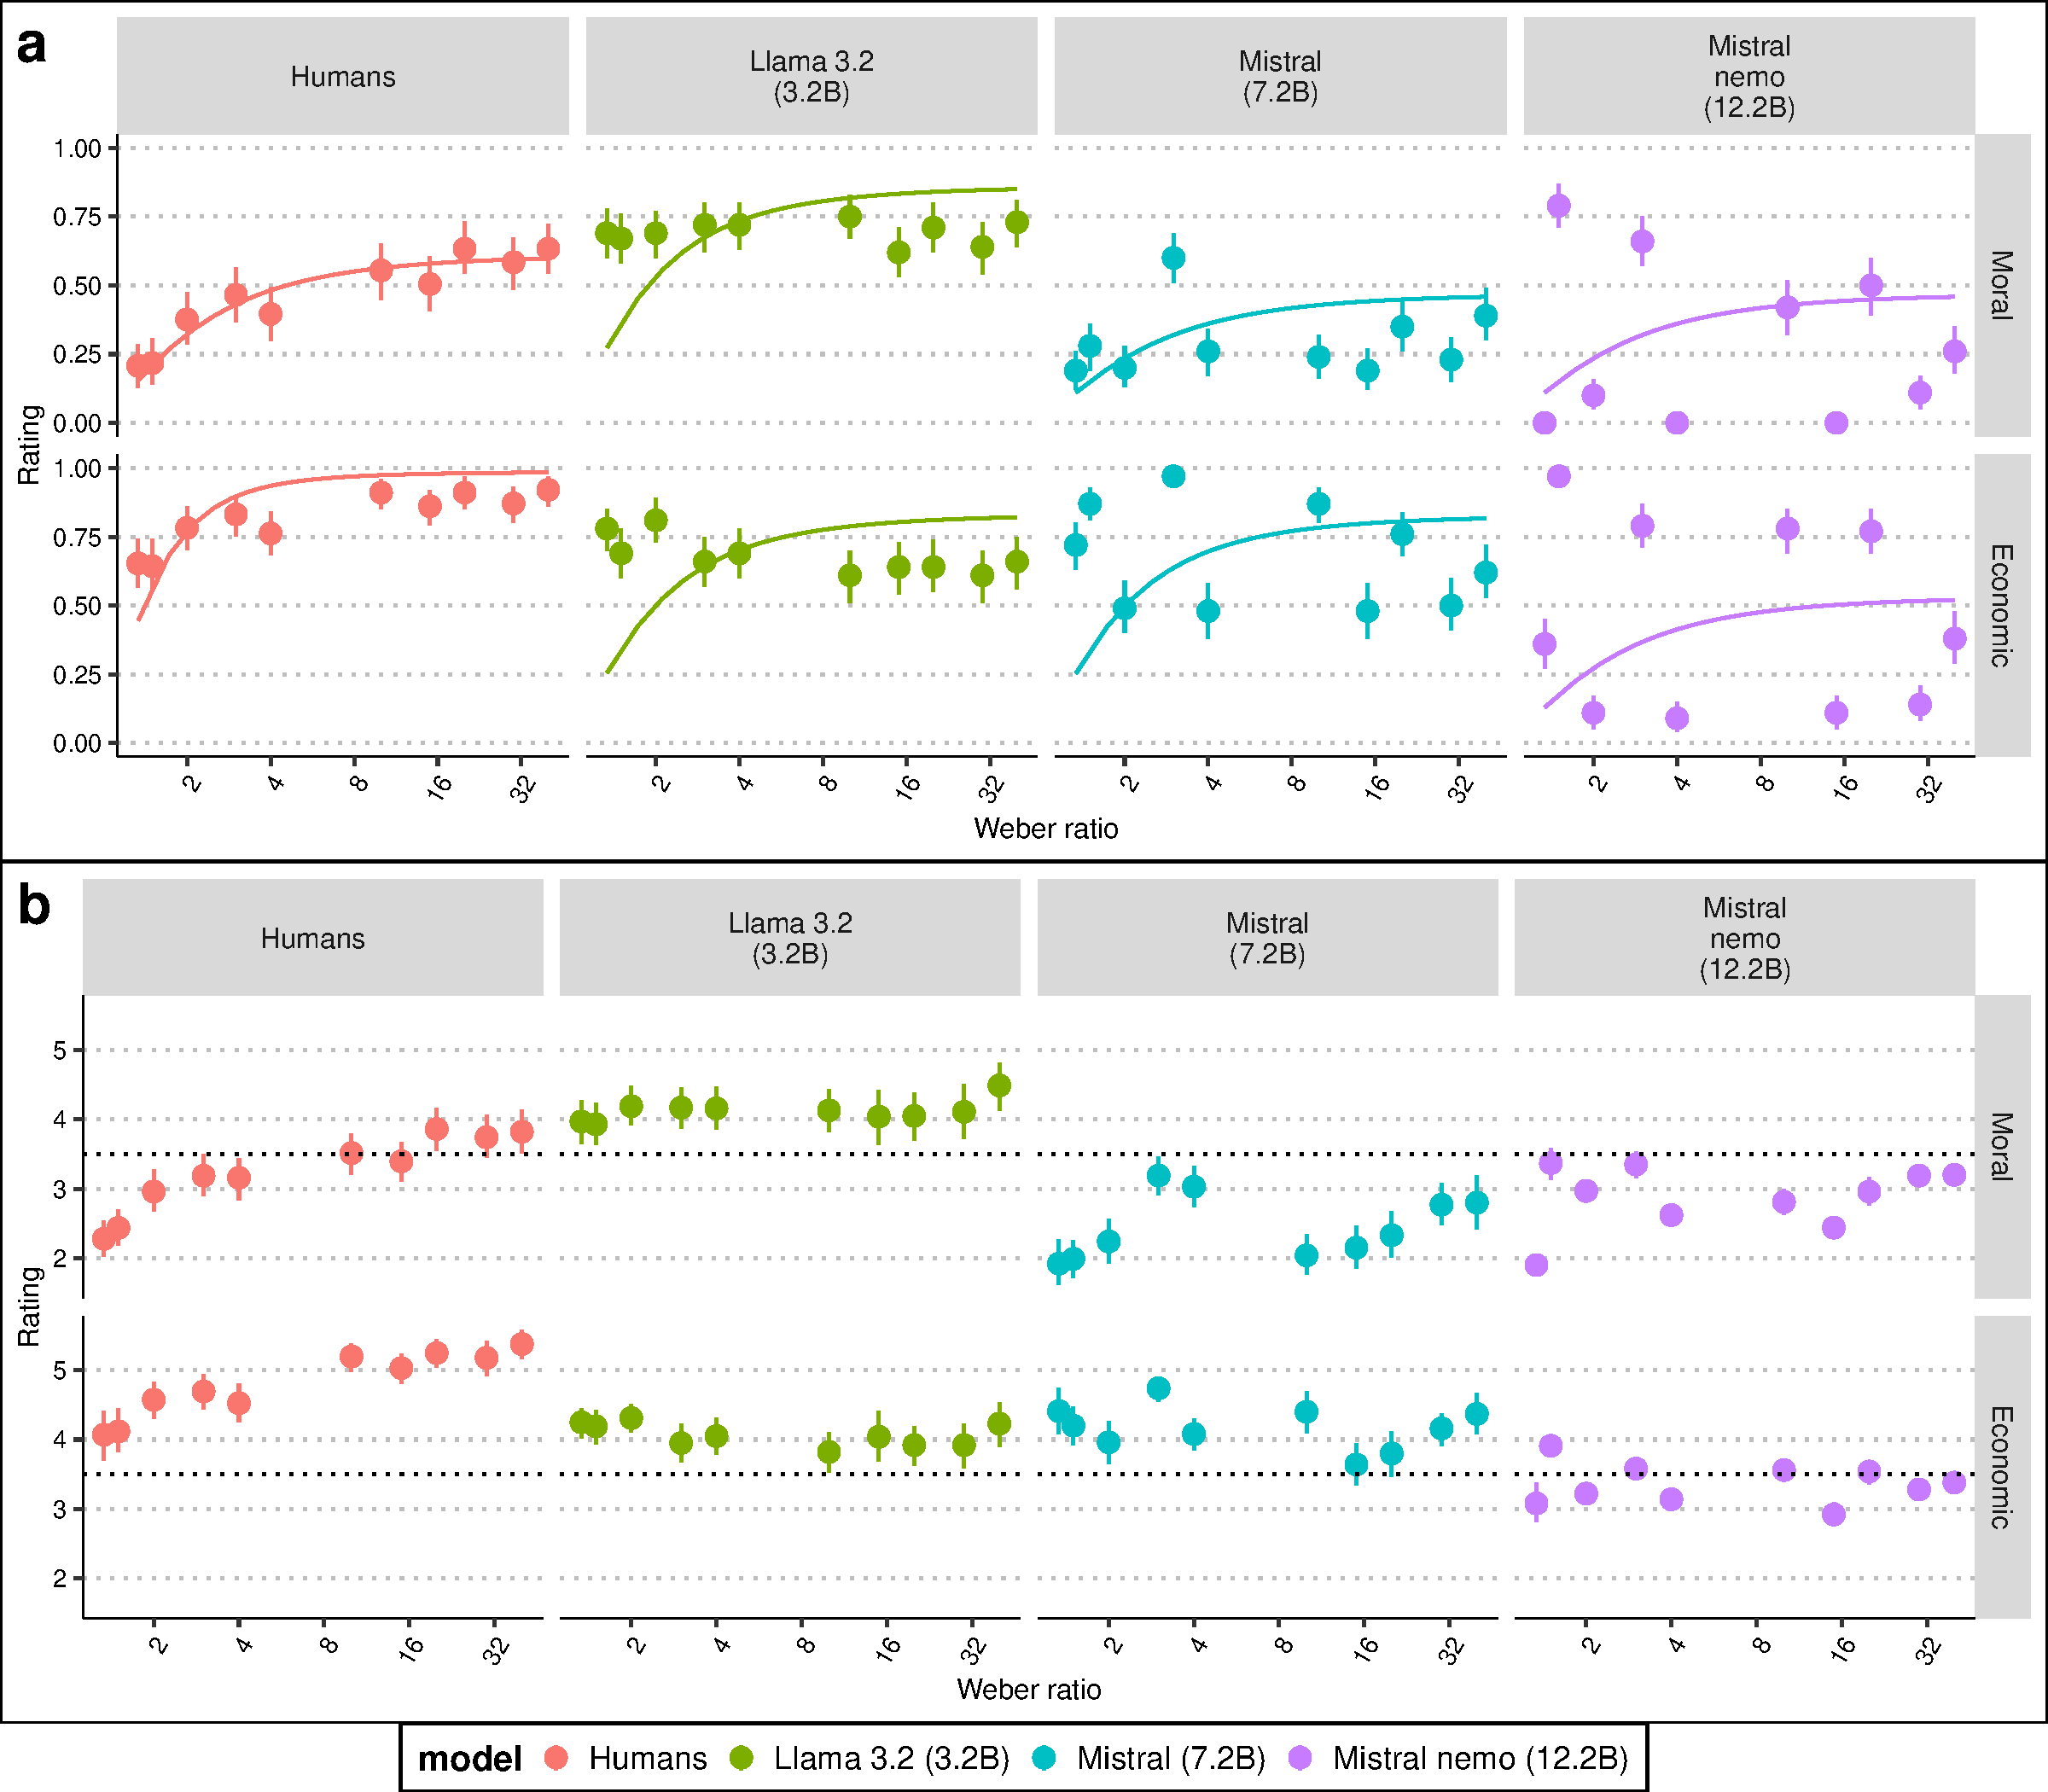
\includegraphics[width=\textwidth,keepaspectratio]{moral_numbers_LLMs_files/figure-latex/plot-llm-results-exp4-ratio-local-1} 

}

\caption{Acceptability of sacrificial decisions as a function of \emph{beneficiary:victim} Weber ratios in Experiment 2 for \emph{local models}. Points represent mean acceptability with 95\% confidence intervals. Curves show psychophysical model fits for the average responses across simulated participants. (a) \emph{Binarized responses} (acceptable/unacceptable) for moral (top) and economic (bottom) scenarios. (b) \emph{Raw} responses on a 6-point scale. Unlike frontier models, local models showed no discernible sensitivity to Weber ratios in either moral or economic scenarios. However, most models showed higher acceptability rates for economic than for moral decisions.}\label{fig:plot-llm-results-exp4-ratio-local}
\end{figure}

In contrast to the frontier models, the (smaller) local models showed no discernible sensitivity to Weber ratios, neither in binary ratings (see Figure \ref{fig:plot-llm-results-exp4-ratio-local}a) nor in raw ratings (see Figure \ref{fig:plot-llm-results-exp4-ratio-local}b). However, most did show higher acceptability rates for economic than for moral decisions.

Accordingly, and as shown in Table \ref{tab:print-fits-exp2}, when fitting the model behavior to our decision model, the noise parameter (\(w\)) was higher in the moral than in the economic condition for most models, with the exception of Llama 3.2 (3.2B), where the two values were comparable.

\paragraph{Summary}\label{summary}

Taken together, these results suggest that LLMs can show some sensitivity to Weber ratios in both moral and economic decisions, at least for large frontier models, but not for smaller local models. Further, most models rated economic sacrifices as more acceptable than moral sacrifices. However, the fit to our psychophysical model was of variable quality.

\clearpage

\subsubsection{Experiment 3}\label{experiment-3}

\paragraph{Frontier models}\label{frontier-models-1}

\begin{figure}

{\centering 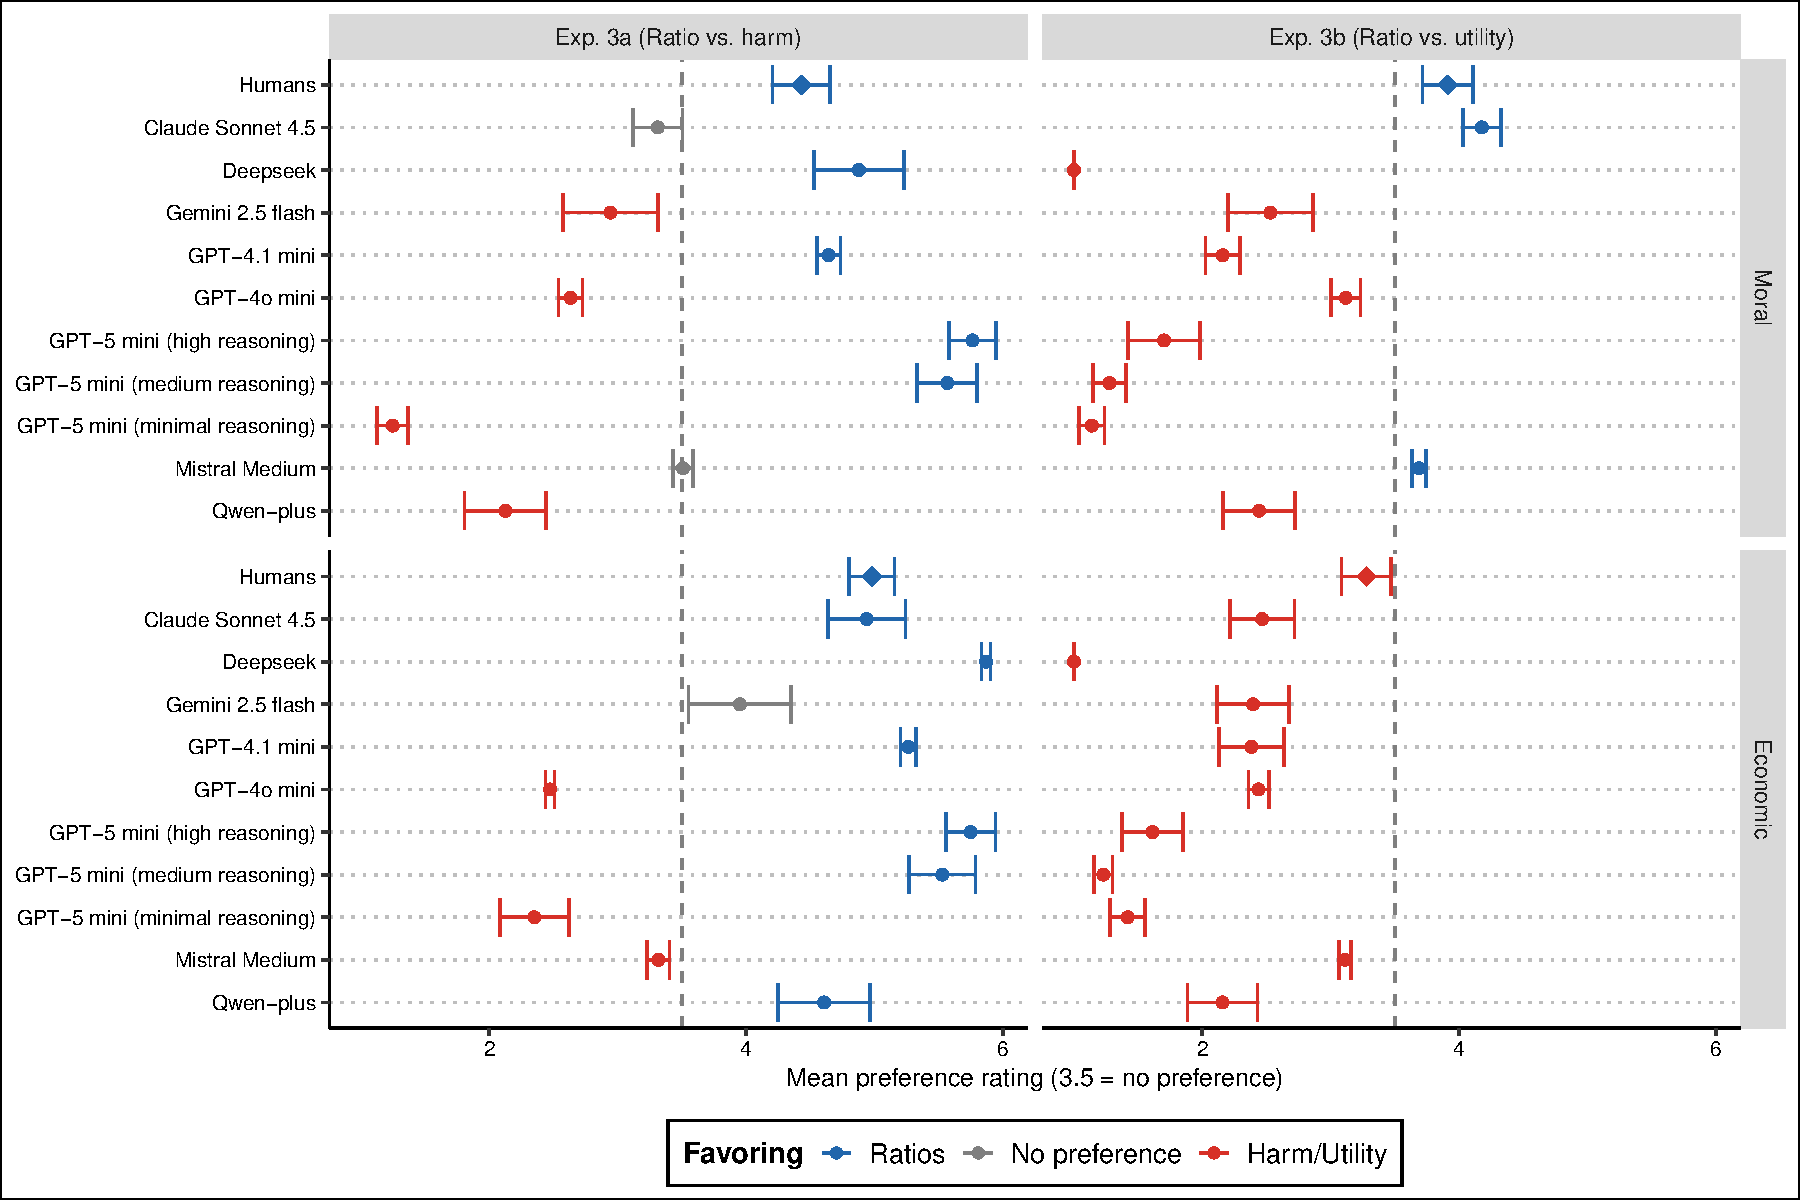
\includegraphics[width=0.8\linewidth]{moral_numbers_LLMs_files/figure-latex/plot-llm-results-exp2-forest-1} 

}

\caption{Forest plot of preferences between high-ratio and alternative options in Experiment 3 for frontier models. Points show mean preference ratings with 95\% confidence intervals. The vertical dashed line at 3.5 indicates no preference; values above favour the high Weber ratio option, values below favour the alternative (low harm in Exp. 3a, high utility in Exp. 3b). Humans are shown as larger diamonds. Colour indicates the significantly favoured option (blue = ratio, red = alternative, grey = no significant preference).}\label{fig:plot-llm-results-exp2-forest}
\end{figure}

\begin{figure}

{\centering 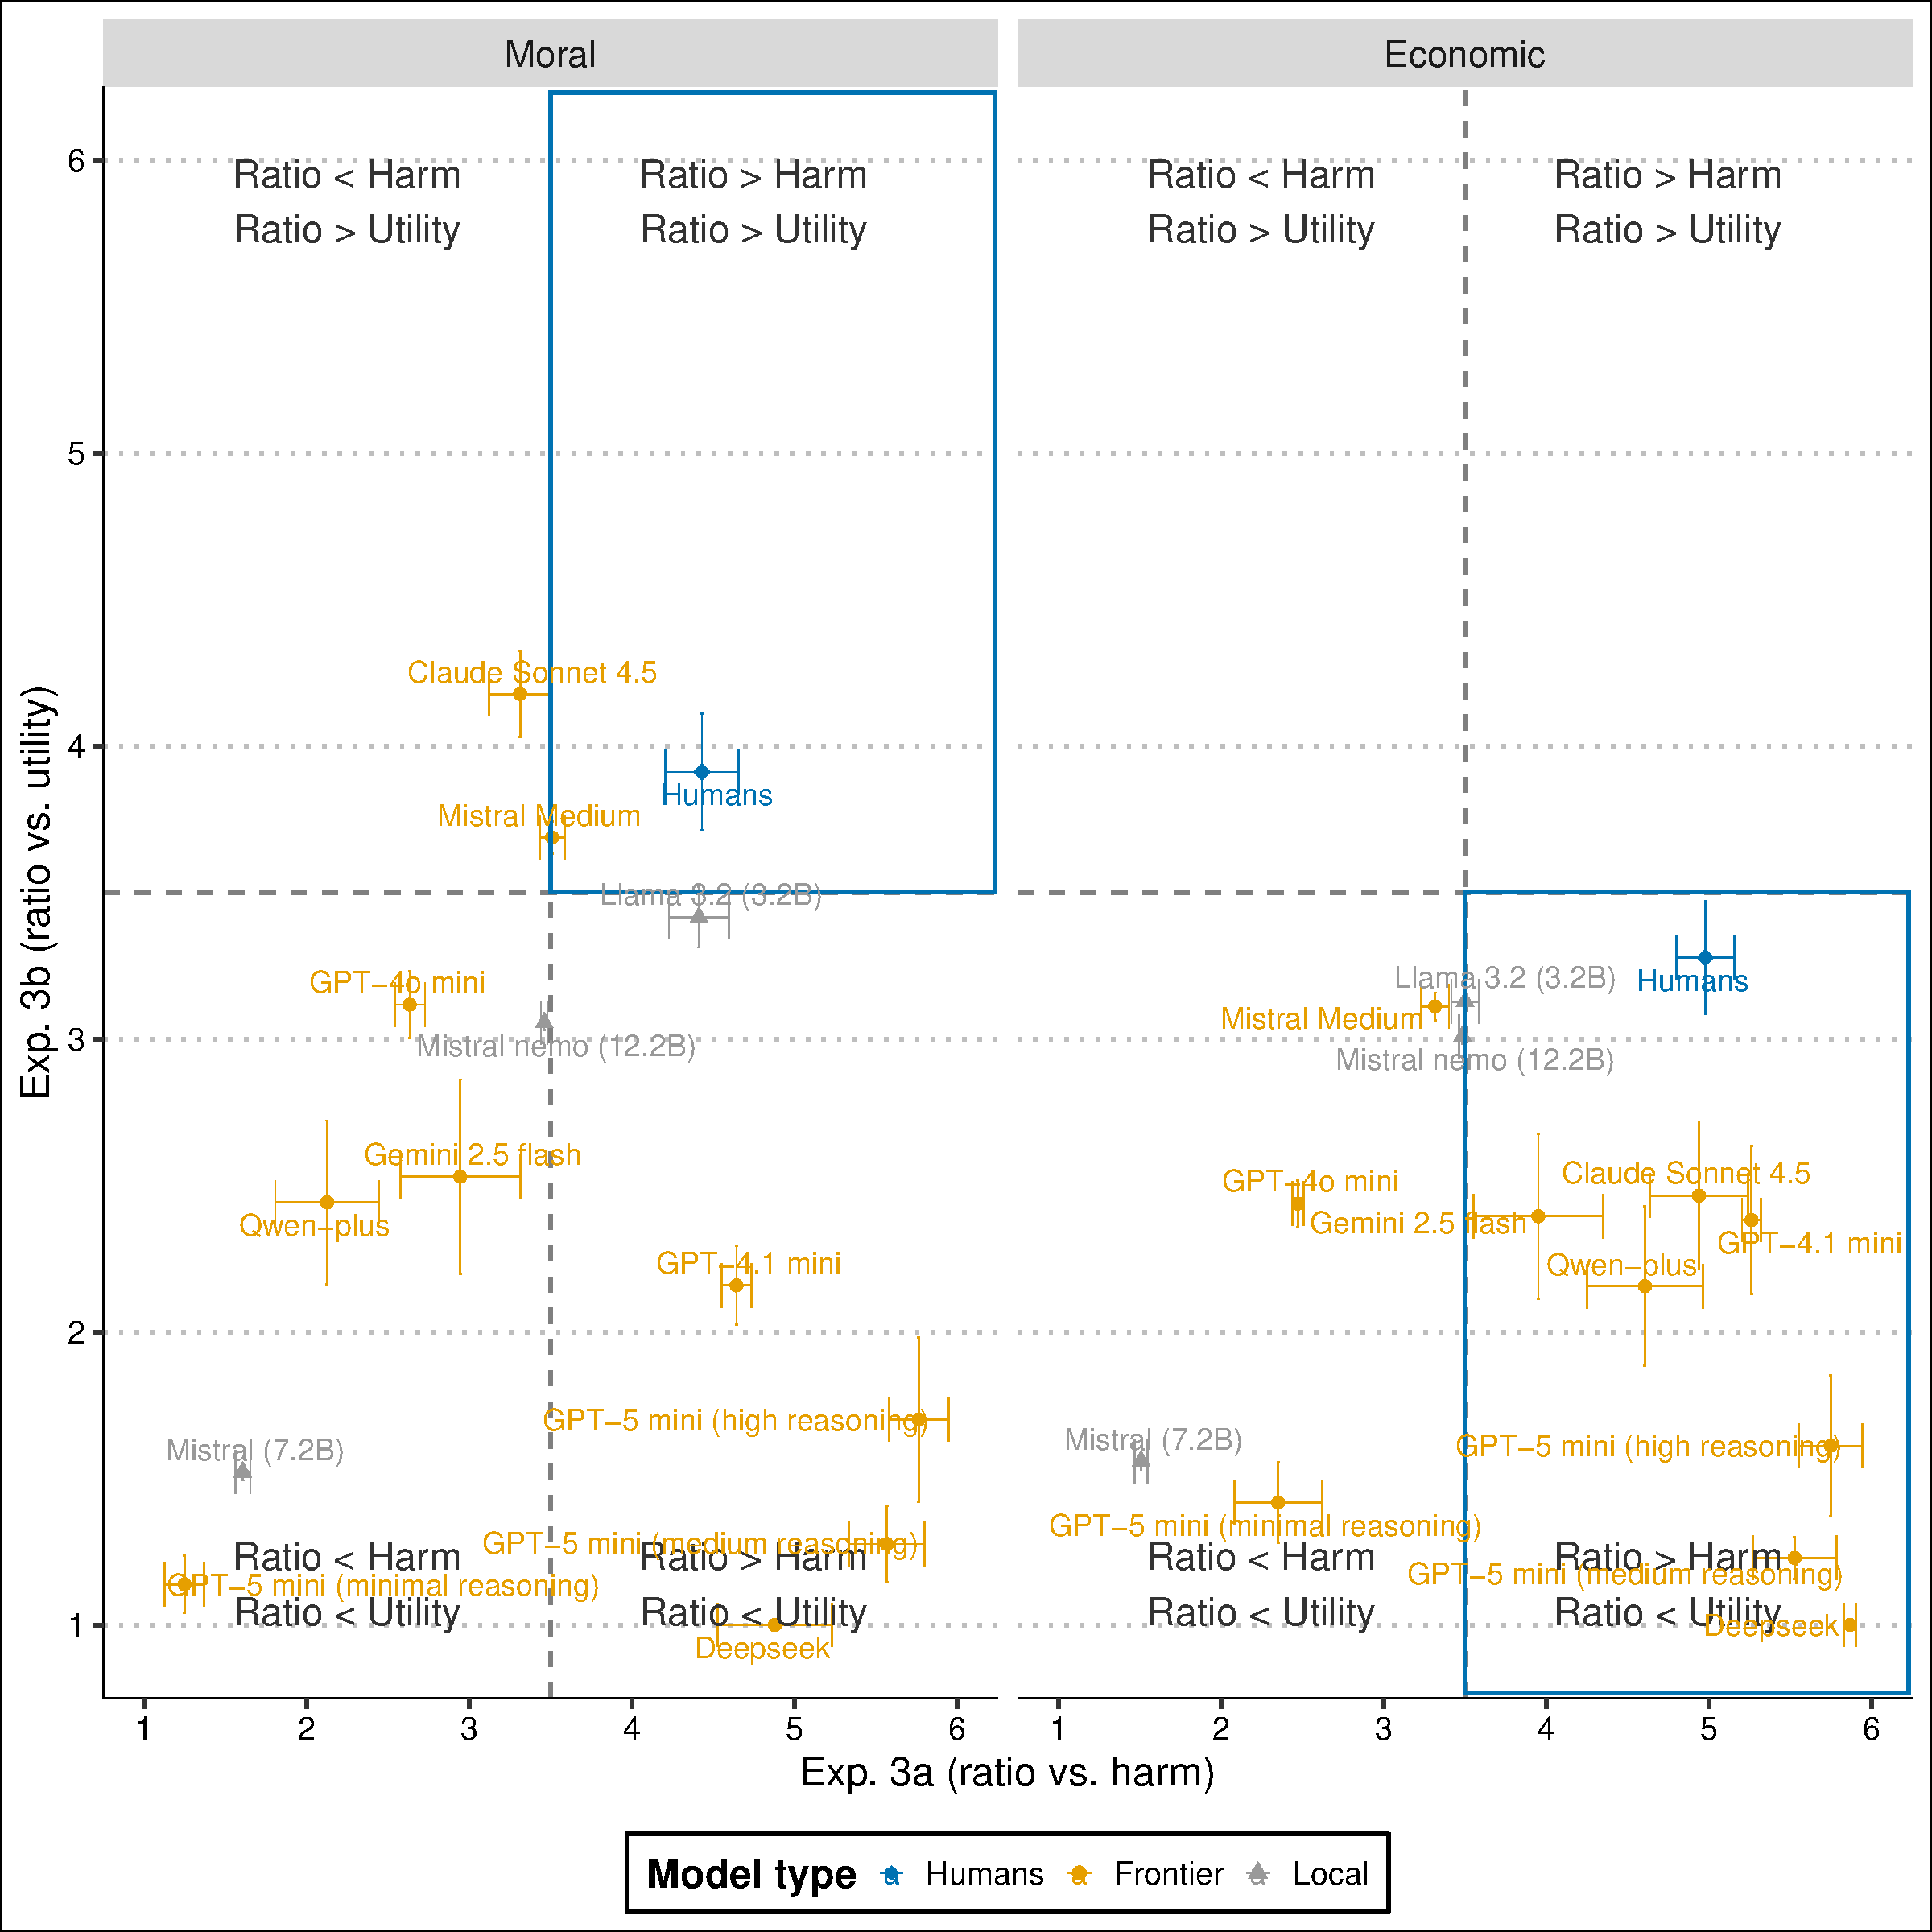
\includegraphics[width=\textwidth,keepaspectratio]{moral_numbers_LLMs_files/figure-latex/plot-llm-exp2-joint-preference-plot-1} 

}

\caption{Joint preference ratings in Experiment 3 for each model and condition. The x-axis shows the mean preference rating in Experiment 3a (ratio vs. harm); the y-axis shows the mean rating in Experiment 3b (ratio vs. utility). Both axes use a 1--6 scale where 3.5 indicates no preference. Error bars show 95\% CIs. Background colours indicate the quadrant: top-right (blue) = ratio preferred in both experiments, the human-like pattern. Colour and shape distinguish humans (red diamond), frontier models (dark circles), and local models (teal triangles). Quadrant labels are placed in the margins.}\label{fig:plot-llm-exp2-joint-preference-plot}
\end{figure}

\begin{figure}

{\centering 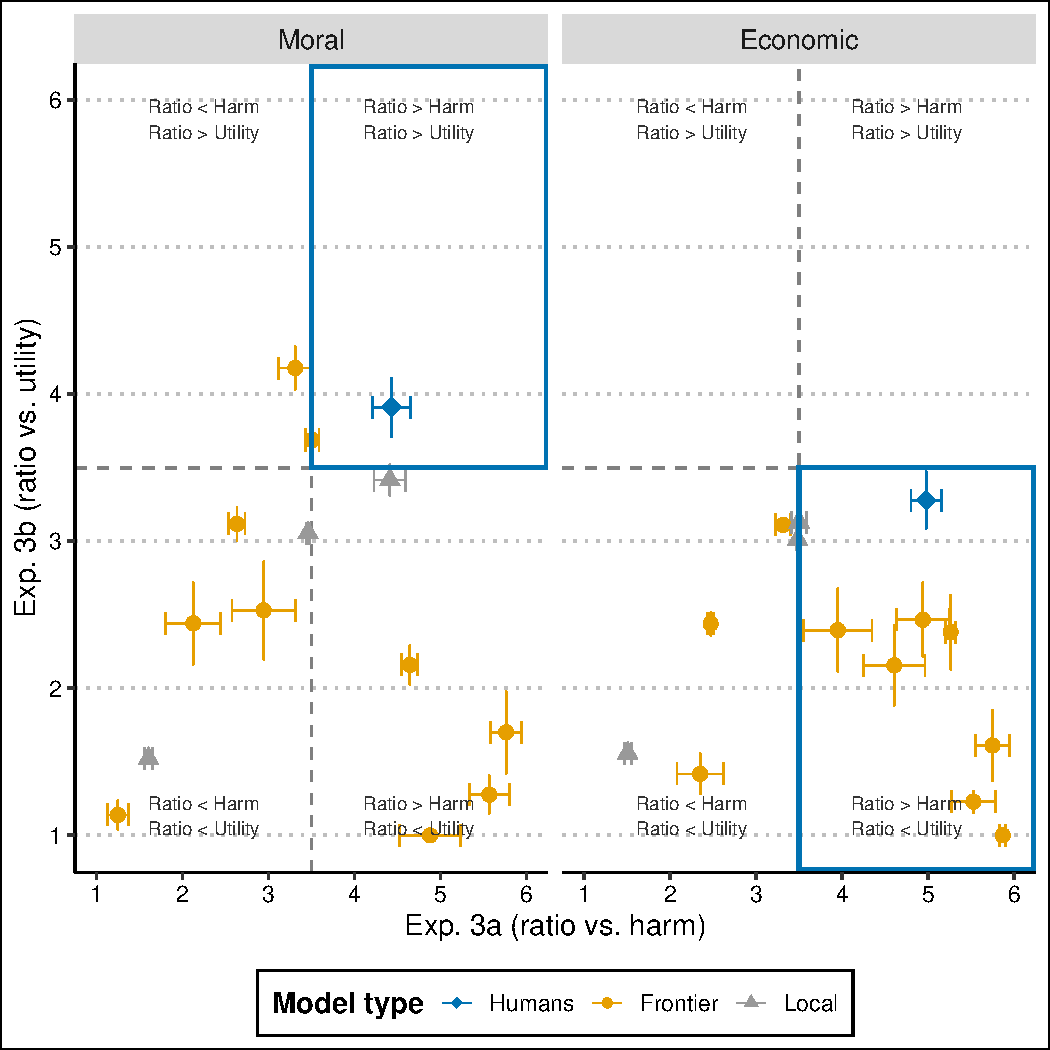
\includegraphics[width=0.8\linewidth]{moral_numbers_LLMs_files/figure-latex/plot-llm-exp2-joint-preference-plot-no-labels-1} 

}

\caption{Joint preference ratings in Experiment 3 for each model and condition. The x-axis shows the mean preference rating in Experiment 3a (ratio vs. harm); the y-axis shows the mean rating in Experiment 3b (ratio vs. utility). Both axes use a 1--6 scale where 3.5 indicates no preference. Error bars show 95\% CIs. Background colours indicate the quadrant: top-right (blue) = ratio preferred in both experiments, the human-like pattern. Colour and shape distinguish humans (red diamond), frontier models (dark circles), and local models (teal triangles). Quadrant labels are placed in the margins. REMOVE THIS, THIS IS SUPPOSED TO BE INCLUDED ONLY IN THE MAIN TEXT}\label{fig:plot-llm-exp2-joint-preference-plot-no-labels}
\end{figure}

In Experiment 3, participants had to choose between two options. In Experiment 3a, one option had a higher \emph{beneficiary:victim} Weber ratio and a higher number of victims (i.e., harm), while the other had a lower \emph{beneficiary:victim} Weber ratio and also lower harm. In Experiment 3b, we similarly pitted Weber ratios against utility. In moral situations, humans prefer to maximize Weber ratios over minimizing harm or maximizing utility. In economic situations, in contrast, they still prioritize Weber ratios over harm, but prioritize utility over Weber ratios.

The results from the LLM simulations are shown in Figures \ref{fig:plot-llm-results-exp2-forest} and \ref{fig:plot-llm-exp2-joint-preference-prepare} (see Table \ref{tab:print-exp2-descriptives-print-details} for detailed results). When pitting Weber ratios against harm in moral situations, four of the frontier models prioritized Weber ratios, four prioritized minimizing harm, while two had no preference. In economic situations, six of the LLMs prioritized Weber ratios, three prioritized minimizing harm, while one had no preference. Thus, only 4 out of 10 models reproduced the human pattern of results in moral situations, and 6 out of 10 in economic situations.

When pitting Weber ratios against utility, eight models prioritized utility in moral situations while two prioritized Weber ratios. In economic situations, all models prioritized utility. Both humans and LLMs thus prioritized utility in economic situations. In contrast, in moral situations, all but two models (Claude-Sonnet 4.5 and Mistral Medium) showed a qualitatively different behavior from humans, and prioritized utility over Weber ratio. However, neither Claude-Sonnet 4.5 nor Mistral Medium showed a preference for Weber ratio over harm, suggesting that they did not account for the human pattern of results either.

In other words, while some models showed a preference for Weber ratios over harm and some a preference for Weber ratios over utility, no model reproduced the human pattern of results.

\begin{longtable}[t]{llrrll}
\caption{\label{tab:print-exp2-descriptives-print-details}Detailed results from Experiment 3. Mean ratings (\emph{M}) with standard errors (\emph{SE}) are shown on a 1-6 scale, where values greater than 3.5 indicate preference for the high Weber ratio option and values smaller 3.5 indicate preference for the alternative option (low harm in Experiment 3a, high utility in Experiment 3b). The p-value tests whether the mean differs from 3.5 (no preference). The \emph{favoring} column indicates which option was significantly preferred. }\\
\toprule
\textbf{Model} & \textbf{Condition} & \textbf{\textit{M}} & \textbf{\textit{SE}} & \textbf{\textit{p}} & \textbf{Favoring}\\
\midrule
\endfirsthead
\caption[]{\label{tab:print-exp2-descriptives-print-details}Detailed results from Experiment 3. Mean ratings (\emph{M}) with standard errors (\emph{SE}) are shown on a 1-6 scale, where values greater than 3.5 indicate preference for the high Weber ratio option and values smaller 3.5 indicate preference for the alternative option (low harm in Experiment 3a, high utility in Experiment 3b). The p-value tests whether the mean differs from 3.5 (no preference). The \emph{favoring} column indicates which option was significantly preferred.  \textit{(continued)}}\\
\toprule
\textbf{Model} & \textbf{Condition} & \textbf{\textit{M}} & \textbf{\textit{SE}} & \textbf{\textit{p}} & \textbf{Favoring}\\
\midrule
\endhead

\endfoot
\bottomrule
\endlastfoot
\addlinespace[0.3em]
\multicolumn{6}{l}{\textbf{\makecell[l]{Humans - Exp. 3a\\(Ratio vs. harm)}}}\\
\cellcolor{gray!10}{\hspace{1em}Humans} & \cellcolor{gray!10}{Moral} & \cellcolor{gray!10}{4.43} & \cellcolor{gray!10}{0.115} & \cellcolor{gray!10}{<0.001} & \cellcolor{gray!10}{Ratios}\\
\hspace{1em}Humans & Economic & 4.98 & 0.091 & <0.001 & Ratios\\
\addlinespace[0.3em]
\multicolumn{6}{l}{\textbf{\makecell[l]{Frontier models - Exp. 3a\\(Ratio vs. harm)}}}\\
\cellcolor{gray!10}{\hspace{1em}Claude Sonnet 4.5} & \cellcolor{gray!10}{Moral} & \cellcolor{gray!10}{3.31} & \cellcolor{gray!10}{0.098} & \cellcolor{gray!10}{0.714} & \cellcolor{gray!10}{}\\
\hspace{1em}Deepseek & Moral & 4.88 & 0.179 & <0.001 & Ratios\\
\cellcolor{gray!10}{\hspace{1em}Gemini 2.5 flash} & \cellcolor{gray!10}{Moral} & \cellcolor{gray!10}{2.94} & \cellcolor{gray!10}{0.188} & \cellcolor{gray!10}{<0.001} & \cellcolor{gray!10}{Harm}\\
\hspace{1em}GPT-4.1 mini & Moral & 4.64 & 0.047 & <0.001 & Ratios\\
\cellcolor{gray!10}{\hspace{1em}GPT-4o mini} & \cellcolor{gray!10}{Moral} & \cellcolor{gray!10}{2.63} & \cellcolor{gray!10}{0.048} & \cellcolor{gray!10}{<0.001} & \cellcolor{gray!10}{Harm}\\
\hspace{1em}GPT-5 mini (high reasoning) & Moral & 5.76 & 0.093 & <0.001 & Ratios\\
\cellcolor{gray!10}{\hspace{1em}GPT-5 mini (medium reasoning)} & \cellcolor{gray!10}{Moral} & \cellcolor{gray!10}{5.57} & \cellcolor{gray!10}{0.119} & \cellcolor{gray!10}{<0.001} & \cellcolor{gray!10}{Ratios}\\
\hspace{1em}GPT-5 mini (minimal reasoning) & Moral & 1.25 & 0.062 & <0.001 & Harm\\
\cellcolor{gray!10}{\hspace{1em}Mistral Medium} & \cellcolor{gray!10}{Moral} & \cellcolor{gray!10}{3.51} & \cellcolor{gray!10}{0.040} & \cellcolor{gray!10}{0.836} & \cellcolor{gray!10}{}\\
\hspace{1em}Qwen-plus & Moral & 2.12 & 0.163 & <0.001 & Harm\\
\cellcolor{gray!10}{\hspace{1em}Claude Sonnet 4.5} & \cellcolor{gray!10}{Economic} & \cellcolor{gray!10}{4.94} & \cellcolor{gray!10}{0.155} & \cellcolor{gray!10}{<0.001} & \cellcolor{gray!10}{Ratios}\\
\hspace{1em}Deepseek & Economic & 5.87 & 0.018 & <0.001 & Ratios\\
\cellcolor{gray!10}{\hspace{1em}Gemini 2.5 flash} & \cellcolor{gray!10}{Economic} & \cellcolor{gray!10}{3.95} & \cellcolor{gray!10}{0.203} & \cellcolor{gray!10}{0.448} & \cellcolor{gray!10}{}\\
\hspace{1em}GPT-4.1 mini & Economic & 5.26 & 0.030 & <0.001 & Ratios\\
\cellcolor{gray!10}{\hspace{1em}GPT-4o mini} & \cellcolor{gray!10}{Economic} & \cellcolor{gray!10}{2.47} & \cellcolor{gray!10}{0.017} & \cellcolor{gray!10}{<0.001} & \cellcolor{gray!10}{Harm}\\
\hspace{1em}GPT-5 mini (high reasoning) & Economic & 5.75 & 0.099 & <0.001 & Ratios\\
\cellcolor{gray!10}{\hspace{1em}GPT-5 mini (medium reasoning)} & \cellcolor{gray!10}{Economic} & \cellcolor{gray!10}{5.53} & \cellcolor{gray!10}{0.132} & \cellcolor{gray!10}{<0.001} & \cellcolor{gray!10}{Ratios}\\
\hspace{1em}GPT-5 mini (minimal reasoning) & Economic & 2.35 & 0.137 & <0.001 & Harm\\
\cellcolor{gray!10}{\hspace{1em}Mistral Medium} & \cellcolor{gray!10}{Economic} & \cellcolor{gray!10}{3.32} & \cellcolor{gray!10}{0.044} & \cellcolor{gray!10}{<0.001} & \cellcolor{gray!10}{Harm}\\
\hspace{1em}Qwen-plus & Economic & 4.61 & 0.182 & 0.009 & Ratios\\
\addlinespace[0.3em]
\multicolumn{6}{l}{\textbf{\makecell[l]{Local models - Exp. 3a\\(Ratio vs. harm)}}}\\
\cellcolor{gray!10}{\hspace{1em}Llama 3.2 (3.2B)} & \cellcolor{gray!10}{Moral} & \cellcolor{gray!10}{4.41} & \cellcolor{gray!10}{0.094} & \cellcolor{gray!10}{<0.001} & \cellcolor{gray!10}{Ratios}\\
\hspace{1em}Mistral (7.2B) & Moral & 1.61 & 0.024 & <0.001 & Harm\\
\cellcolor{gray!10}{\hspace{1em}Mistral nemo (12.2B)} & \cellcolor{gray!10}{Moral} & \cellcolor{gray!10}{3.46} & \cellcolor{gray!10}{0.010} & \cellcolor{gray!10}{<0.001} & \cellcolor{gray!10}{Harm}\\
\hspace{1em}Llama 3.2 (3.2B) & Economic & 3.50 & 0.043 & 0.123 & \\
\cellcolor{gray!10}{\hspace{1em}Mistral (7.2B)} & \cellcolor{gray!10}{Economic} & \cellcolor{gray!10}{1.51} & \cellcolor{gray!10}{0.021} & \cellcolor{gray!10}{<0.001} & \cellcolor{gray!10}{Harm}\\
\hspace{1em}Mistral nemo (12.2B) & Economic & 3.48 & 0.010 & 0.125 & \\
\addlinespace[0.3em]
\multicolumn{6}{l}{\textbf{\makecell[l]{Humans - Exp. 3b\\(Ratio vs. utility)}}}\\
\cellcolor{gray!10}{\hspace{1em}Humans} & \cellcolor{gray!10}{Moral} & \cellcolor{gray!10}{3.91} & \cellcolor{gray!10}{0.101} & \cellcolor{gray!10}{<0.001} & \cellcolor{gray!10}{Ratios}\\
\hspace{1em}Humans & Economic & 3.28 & 0.099 & 0.033 & Utility\\
\addlinespace[0.3em]
\multicolumn{6}{l}{\textbf{\makecell[l]{Frontier models - Exp. 3b\\(Ratio vs. utility)}}}\\
\cellcolor{gray!10}{\hspace{1em}Claude Sonnet 4.5} & \cellcolor{gray!10}{Moral} & \cellcolor{gray!10}{4.18} & \cellcolor{gray!10}{0.075} & \cellcolor{gray!10}{<0.001} & \cellcolor{gray!10}{Ratios}\\
\hspace{1em}Deepseek & Moral & 1.00 & 0.000 & <0.001 & Utility\\
\cellcolor{gray!10}{\hspace{1em}Gemini 2.5 flash} & \cellcolor{gray!10}{Moral} & \cellcolor{gray!10}{2.53} & \cellcolor{gray!10}{0.169} & \cellcolor{gray!10}{<0.001} & \cellcolor{gray!10}{Utility}\\
\hspace{1em}GPT-4.1 mini & Moral & 2.16 & 0.068 & <0.001 & Utility\\
\cellcolor{gray!10}{\hspace{1em}GPT-4o mini} & \cellcolor{gray!10}{Moral} & \cellcolor{gray!10}{3.12} & \cellcolor{gray!10}{0.059} & \cellcolor{gray!10}{<0.001} & \cellcolor{gray!10}{Utility}\\
\hspace{1em}GPT-5 mini (high reasoning) & Moral & 1.70 & 0.143 & <0.001 & Utility\\
\cellcolor{gray!10}{\hspace{1em}GPT-5 mini (medium reasoning)} & \cellcolor{gray!10}{Moral} & \cellcolor{gray!10}{1.28} & \cellcolor{gray!10}{0.066} & \cellcolor{gray!10}{<0.001} & \cellcolor{gray!10}{Utility}\\
\hspace{1em}GPT-5 mini (minimal reasoning) & Moral & 1.14 & 0.050 & <0.001 & Utility\\
\cellcolor{gray!10}{\hspace{1em}Mistral Medium} & \cellcolor{gray!10}{Moral} & \cellcolor{gray!10}{3.69} & \cellcolor{gray!10}{0.028} & \cellcolor{gray!10}{<0.001} & \cellcolor{gray!10}{Ratios}\\
\hspace{1em}Qwen-plus & Moral & 2.44 & 0.143 & <0.001 & Utility\\
\cellcolor{gray!10}{\hspace{1em}Claude Sonnet 4.5} & \cellcolor{gray!10}{Economic} & \cellcolor{gray!10}{2.47} & \cellcolor{gray!10}{0.128} & \cellcolor{gray!10}{<0.001} & \cellcolor{gray!10}{Utility}\\
\hspace{1em}Deepseek & Economic & 1.00 & 0.000 & <0.001 & Utility\\
\cellcolor{gray!10}{\hspace{1em}Gemini 2.5 flash} & \cellcolor{gray!10}{Economic} & \cellcolor{gray!10}{2.40} & \cellcolor{gray!10}{0.144} & \cellcolor{gray!10}{<0.001} & \cellcolor{gray!10}{Utility}\\
\hspace{1em}GPT-4.1 mini & Economic & 2.38 & 0.129 & <0.001 & Utility\\
\cellcolor{gray!10}{\hspace{1em}GPT-4o mini} & \cellcolor{gray!10}{Economic} & \cellcolor{gray!10}{2.44} & \cellcolor{gray!10}{0.041} & \cellcolor{gray!10}{<0.001} & \cellcolor{gray!10}{Utility}\\
\hspace{1em}GPT-5 mini (high reasoning) & Economic & 1.61 & 0.122 & <0.001 & Utility\\
\cellcolor{gray!10}{\hspace{1em}GPT-5 mini (medium reasoning)} & \cellcolor{gray!10}{Economic} & \cellcolor{gray!10}{1.23} & \cellcolor{gray!10}{0.037} & \cellcolor{gray!10}{<0.001} & \cellcolor{gray!10}{Utility}\\
\hspace{1em}GPT-5 mini (minimal reasoning) & Economic & 1.42 & 0.070 & <0.001 & Utility\\
\cellcolor{gray!10}{\hspace{1em}Mistral Medium} & \cellcolor{gray!10}{Economic} & \cellcolor{gray!10}{3.11} & \cellcolor{gray!10}{0.024} & \cellcolor{gray!10}{<0.001} & \cellcolor{gray!10}{Utility}\\
\hspace{1em}Qwen-plus & Economic & 2.16 & 0.139 & <0.001 & Utility\\
\addlinespace[0.3em]
\multicolumn{6}{l}{\textbf{\makecell[l]{Local models - Exp. 3b\\(Ratio vs. utility)}}}\\
\cellcolor{gray!10}{\hspace{1em}Llama 3.2 (3.2B)} & \cellcolor{gray!10}{Moral} & \cellcolor{gray!10}{3.42} & \cellcolor{gray!10}{0.053} & \cellcolor{gray!10}{<0.001} & \cellcolor{gray!10}{Utility}\\
\hspace{1em}Mistral (7.2B) & Moral & 1.52 & 0.015 & <0.001 & Utility\\
\cellcolor{gray!10}{\hspace{1em}Mistral nemo (12.2B)} & \cellcolor{gray!10}{Moral} & \cellcolor{gray!10}{3.06} & \cellcolor{gray!10}{0.013} & \cellcolor{gray!10}{<0.001} & \cellcolor{gray!10}{Utility}\\
\hspace{1em}Llama 3.2 (3.2B) & Economic & 3.13 & 0.035 & <0.001 & Utility\\
\cellcolor{gray!10}{\hspace{1em}Mistral (7.2B)} & \cellcolor{gray!10}{Economic} & \cellcolor{gray!10}{1.56} & \cellcolor{gray!10}{0.015} & \cellcolor{gray!10}{<0.001} & \cellcolor{gray!10}{Utility}\\
\hspace{1em}Mistral nemo (12.2B) & Economic & 3.01 & 0.013 & <0.001 & Utility\\*
\end{longtable}

\clearpage

\paragraph{Local models}\label{local-models-1}

\begin{figure}

{\centering 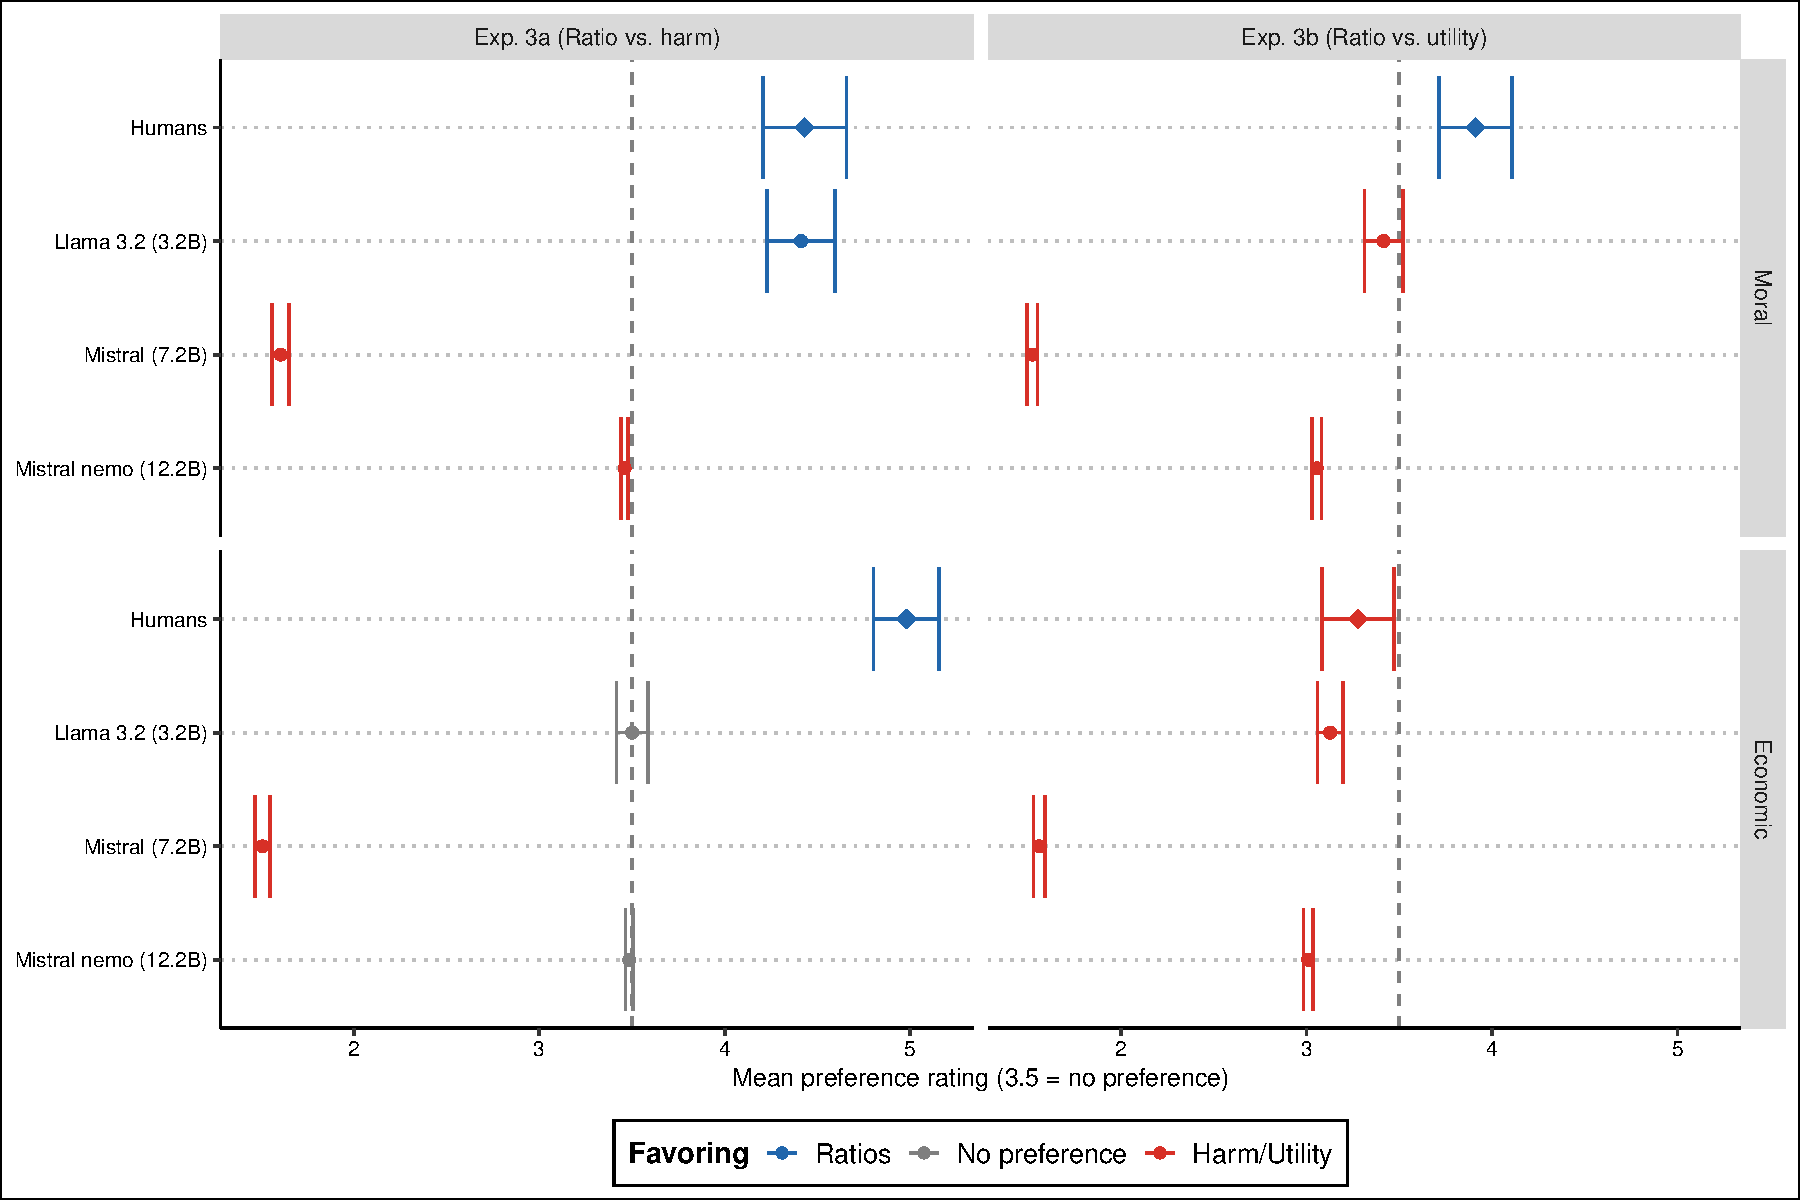
\includegraphics[width=0.8\linewidth]{moral_numbers_LLMs_files/figure-latex/plot-llm-results-exp2-local-forest-1} 

}

\caption{Forest plot of preferences between high-ratio and alternative options in Experiment 3 for local models. Points show mean preference ratings with 95\% confidence intervals. The vertical dashed line at 3.5 indicates no preference; values above favour the high Weber ratio option, values below favour the alternative (low harm in Exp. 3a, high utility in Exp. 3b). Humans are shown as larger diamonds. Colour indicates the significantly favoured option (blue = ratio, red = alternative, grey = no significant preference).}\label{fig:plot-llm-results-exp2-local-forest}
\end{figure}

When considering (smaller) local LLMs, one model preferred Weber ratios over harm in moral situations, while two preferred harm over Weber ratios. In economic situations, one model preferred harm over Weber ratios, while two had no preference. When pitting ratios against utility, all models prioritized utility in both the moral and economic situations.

\paragraph{Summary}\label{summary-1}

In Experiment 3, the LLMs showed qualitatively different behavior. No model replicate the human preference for \emph{beneficiary:victim} ratios over both harm and utility in moral situation, combined with a preference for \emph{beneficiary:victim} ratios over harm, and utility over \emph{beneficiary:victim} ratios in economic situatinos.

Many of the LLMs were much more sensitive to harm than humans. While humans prioritized Weber ratios over harm, half of the frontier LLMs prioritized harm in moral situations, while a third prioritized harm in economic situations.

The LLMs also failed to replicate the preference for Weber ratios over utility in moral situations, with all but 2 models prioritizing utility, which also showed no preference for Weber ratios over harm. However, like humans, the LLMs prioritized utility in economic situations.

\clearpage

\subsubsection{Experiment 6}\label{experiment-6}

Experiment 6 assessed how acceptability ratings depend on \emph{beneficiary:victim} ratios when the deaths of the victims and the beneficiaries are equally salient vs.~when the deaths of the victims are made more vivid and salient. Our critical measure is the risk ratio comparing acceptability rates when the deaths of the victims are vividly portrayed versus when they are presented with the same neutral language as the beneficiaries, \(\mathrm{RR}= \frac{P_{\text{acceptable, vivid}}}{P_{\text{acceptable, neutral}}}\). In humans, this risk ratio is positively correlated with the \emph{beneficiary:victim} Weber ratio, suggesting that the effect of victim salience decreases for higher Weber ratios.

\paragraph{Frontier models}\label{frontier-models-2}

\begin{figure}

{\centering 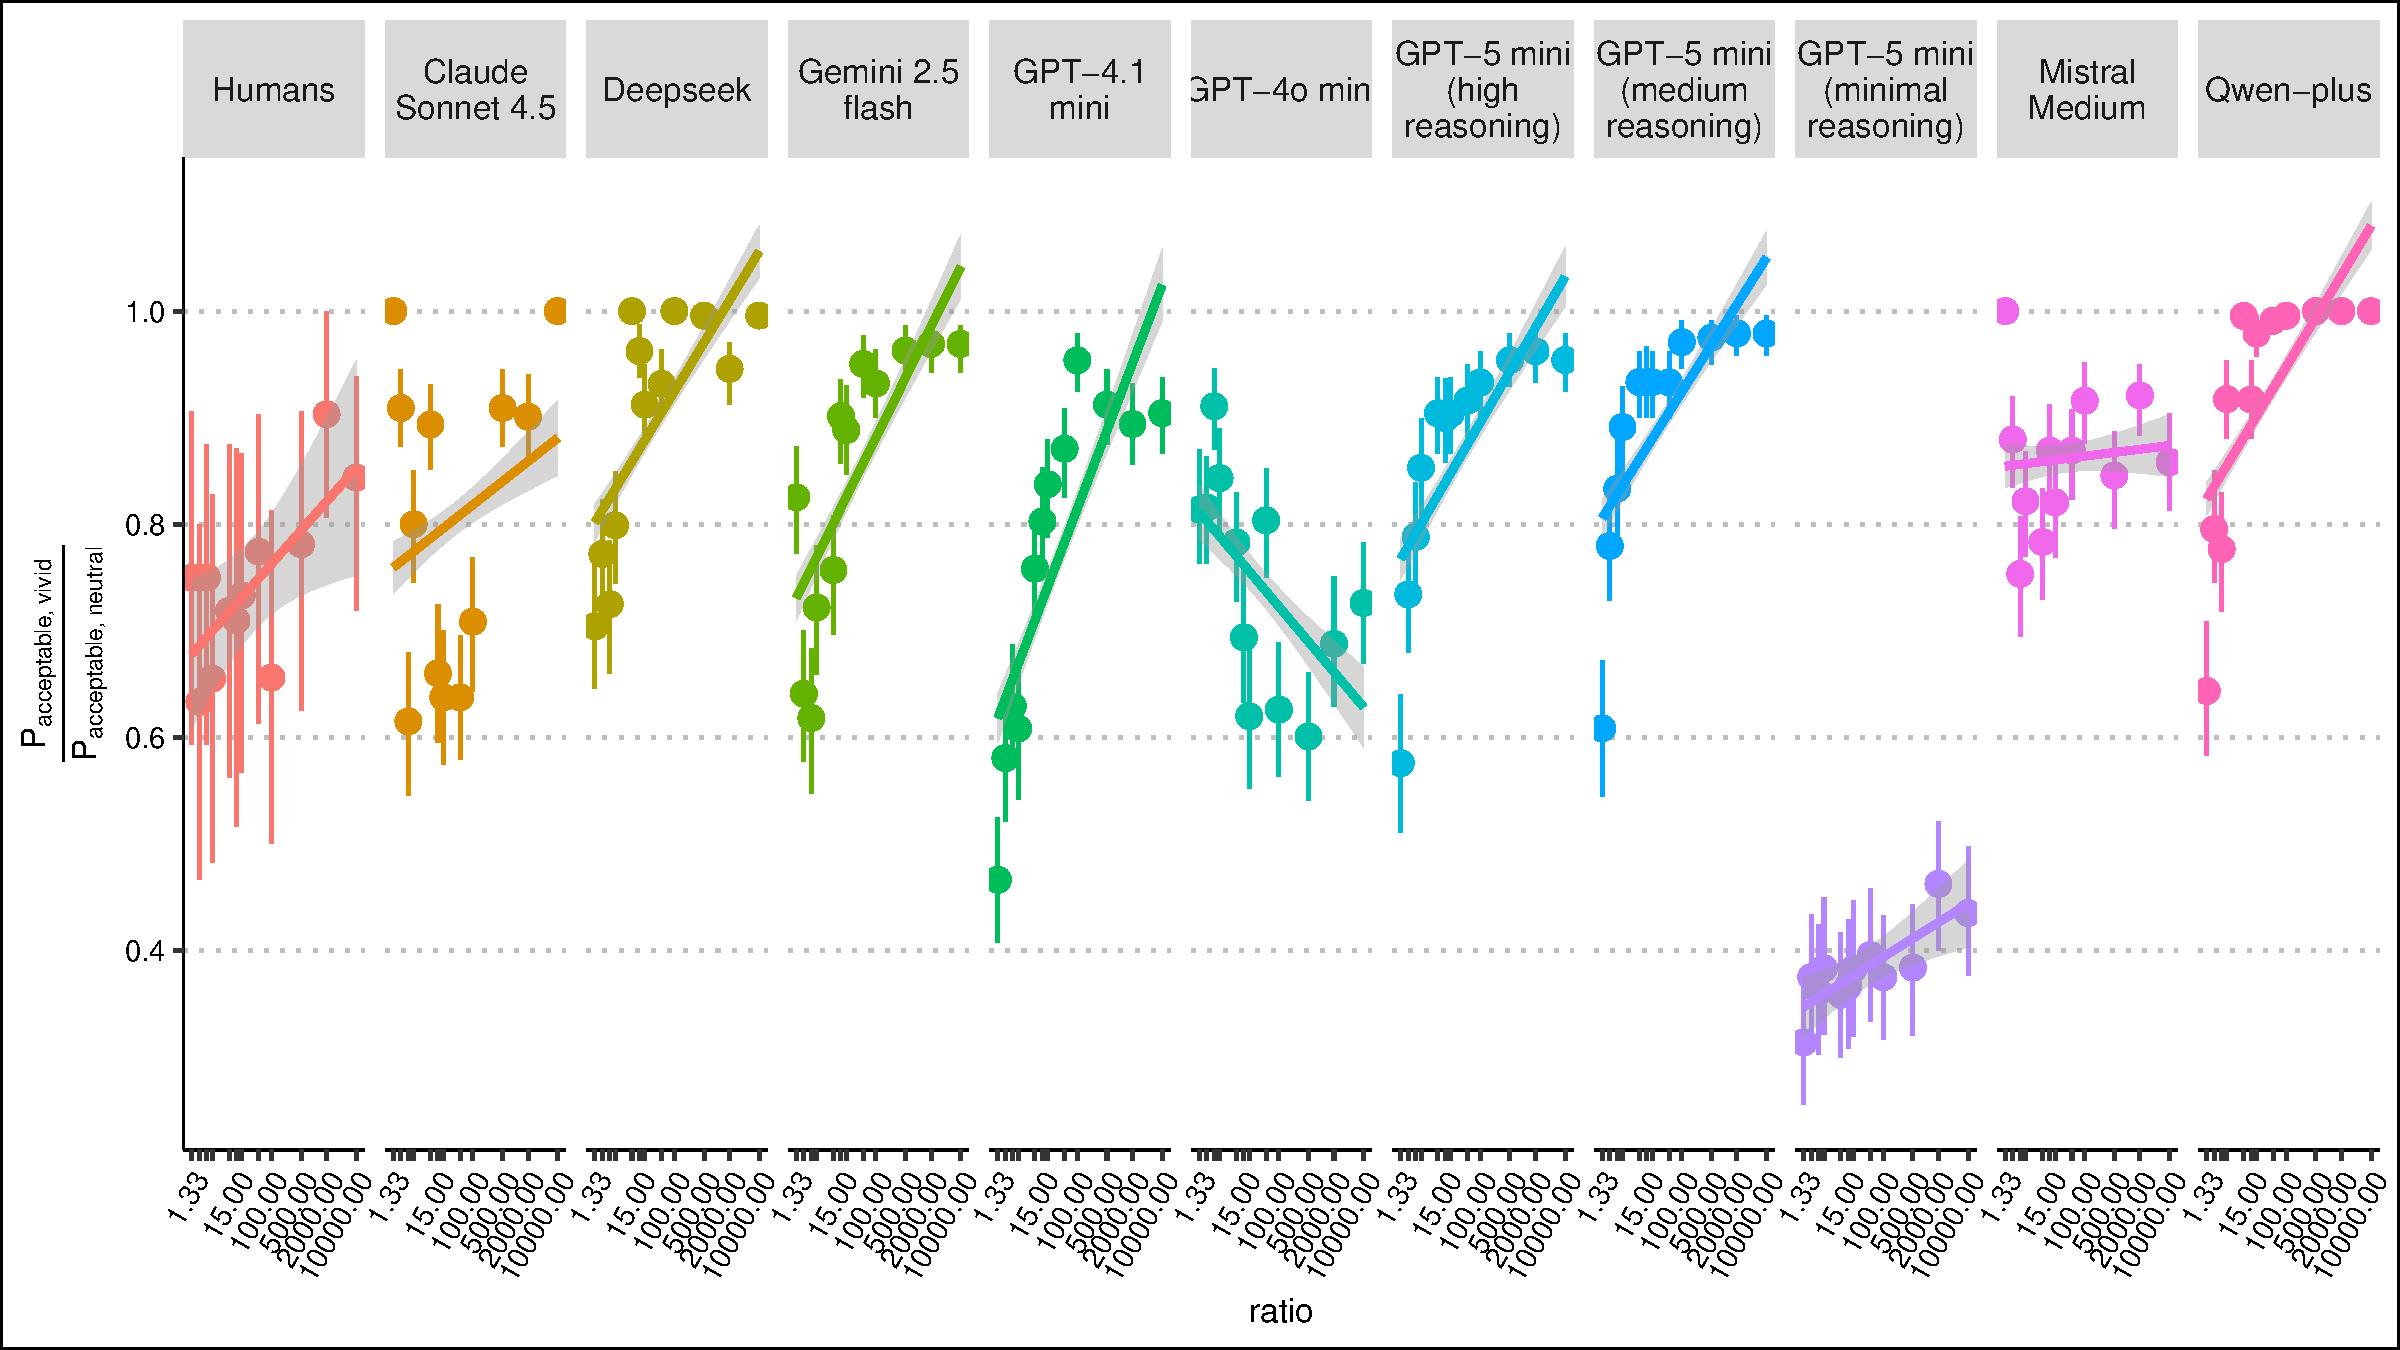
\includegraphics[width=\textwidth,keepaspectratio]{moral_numbers_LLMs_files/figure-latex/exp11-models-relative-risk-plot-cloud-1} 

}

\caption{Risk ratio of acceptability judgements as a function of \emph{beneficiary:victim} Weber ratio in Experiment 6 for frontier models. The risk ratio compares acceptability rates when victims' deaths were portrayed vividly or in the same neutral language as the beneficiaries' deaths, $\mathrm{RR}= \frac{P_{\text{acceptable, vivid}}}{P_{\text{acceptable, neutral}}}$. Points show mean risk ratios with 95\% confidence intervals. Regression lines show the relationship between Weber ratio and risk ratio. In humans, higher Weber ratios are associated with higher risk ratios, indicating that the effect of the salience of the victims' deaths portrayals is reduced for higher \emph{beneficiary:victim} ratios. Seven frontier models reproduced this positive correlation, one showed a negative correlation (GPT-4o mini), and two showed no correlation (Claude Sonnet 4.5, Mistral Medium).}\label{fig:exp11-models-relative-risk-plot-cloud}
\end{figure}

The results for the frontier models are shown in Figure \ref{fig:exp11-models-relative-risk-plot-cloud} and Table \ref{tab:relative-risk-correlations-llm-print}. Seven models showed the same positive correlation as humans, one showed a negative correlation (GPT-4o mini), and two showed no correlation (Claude-Sonnet-4.5 and Mistral Medium).

\begin{longtable}[t]{lrll}
\caption{\label{tab:relative-risk-correlations-llm-print}Correlations between Weber ratio and risk ratio in Experiment 6. The risk ratio $\mathrm{RR}= \frac{P_{\text{acceptable, vivid}}}{P_{\text{acceptable, neutral}}}$ measures how much the saliency of the victims' death reduces acceptability judgments. Positive correlations indicate that this effect diminishes at higher Weber ratios (matching human behavior). Correlation coefficients ($\rho$), p-values (p), and significance levels (sig: * p < .05, ** p < .01, *** p < .001, ns = not significant) are shown. Most frontier models showed significant positive correlations, while local models showed negative or no correlations.}\\
\toprule
\textbf{model} & \textbf{$\rho$} & \textbf{p} & \textbf{sig}\\
\midrule
\addlinespace[0.3em]
\multicolumn{4}{l}{\textbf{Frontier models}}\\
\hspace{1em}Humans & 0.110 & 0.041 & \vphantom{1} *\\
\hspace{1em}Claude Sonnet 4.5 & 0.018 & 0.370 & ns\\
\hspace{1em}Deepseek & 0.290 & <0.001 & ***\\
\hspace{1em}Gemini 2.5 flash & 0.280 & <0.001 & ***\\
\hspace{1em}GPT-4.1 mini & 0.330 & <0.001 & ***\\
\hspace{1em}GPT-4o mini & -0.150 & <0.001 & ***\\
\hspace{1em}GPT-5 mini (high reasoning) & 0.270 & <0.001 & ***\\
\hspace{1em}GPT-5 mini (medium reasoning) & 0.290 & <0.001 & ***\\
\hspace{1em}GPT-5 mini (minimal reasoning) & 0.059 & 0.002 & **\\
\hspace{1em}Mistral Medium & 0.005 & 0.786 & ns\\
\hspace{1em}Qwen-plus & 0.340 & <0.001 & ***\\
\addlinespace[0.3em]
\multicolumn{4}{l}{\textbf{Local models}}\\
\hspace{1em}Humans & 0.110 & 0.041 & *\\
\hspace{1em}Llama 3.2 (3.2B) & -0.036 & 0.064 & .\\
\hspace{1em}Mistral (7.2B) & -0.040 & 0.038 & *\\
\hspace{1em}Mistral nemo (12.2B) & -0.012 & 0.525 & ns\\
\bottomrule
\end{longtable}

We also present the acceptability ratings and model fits in Figure \ref{fig:plot-llm-results-exp11-ratio-bin} and Table \ref{tab:print-fits-exp11}, respectively.

\begin{figure}

{\centering 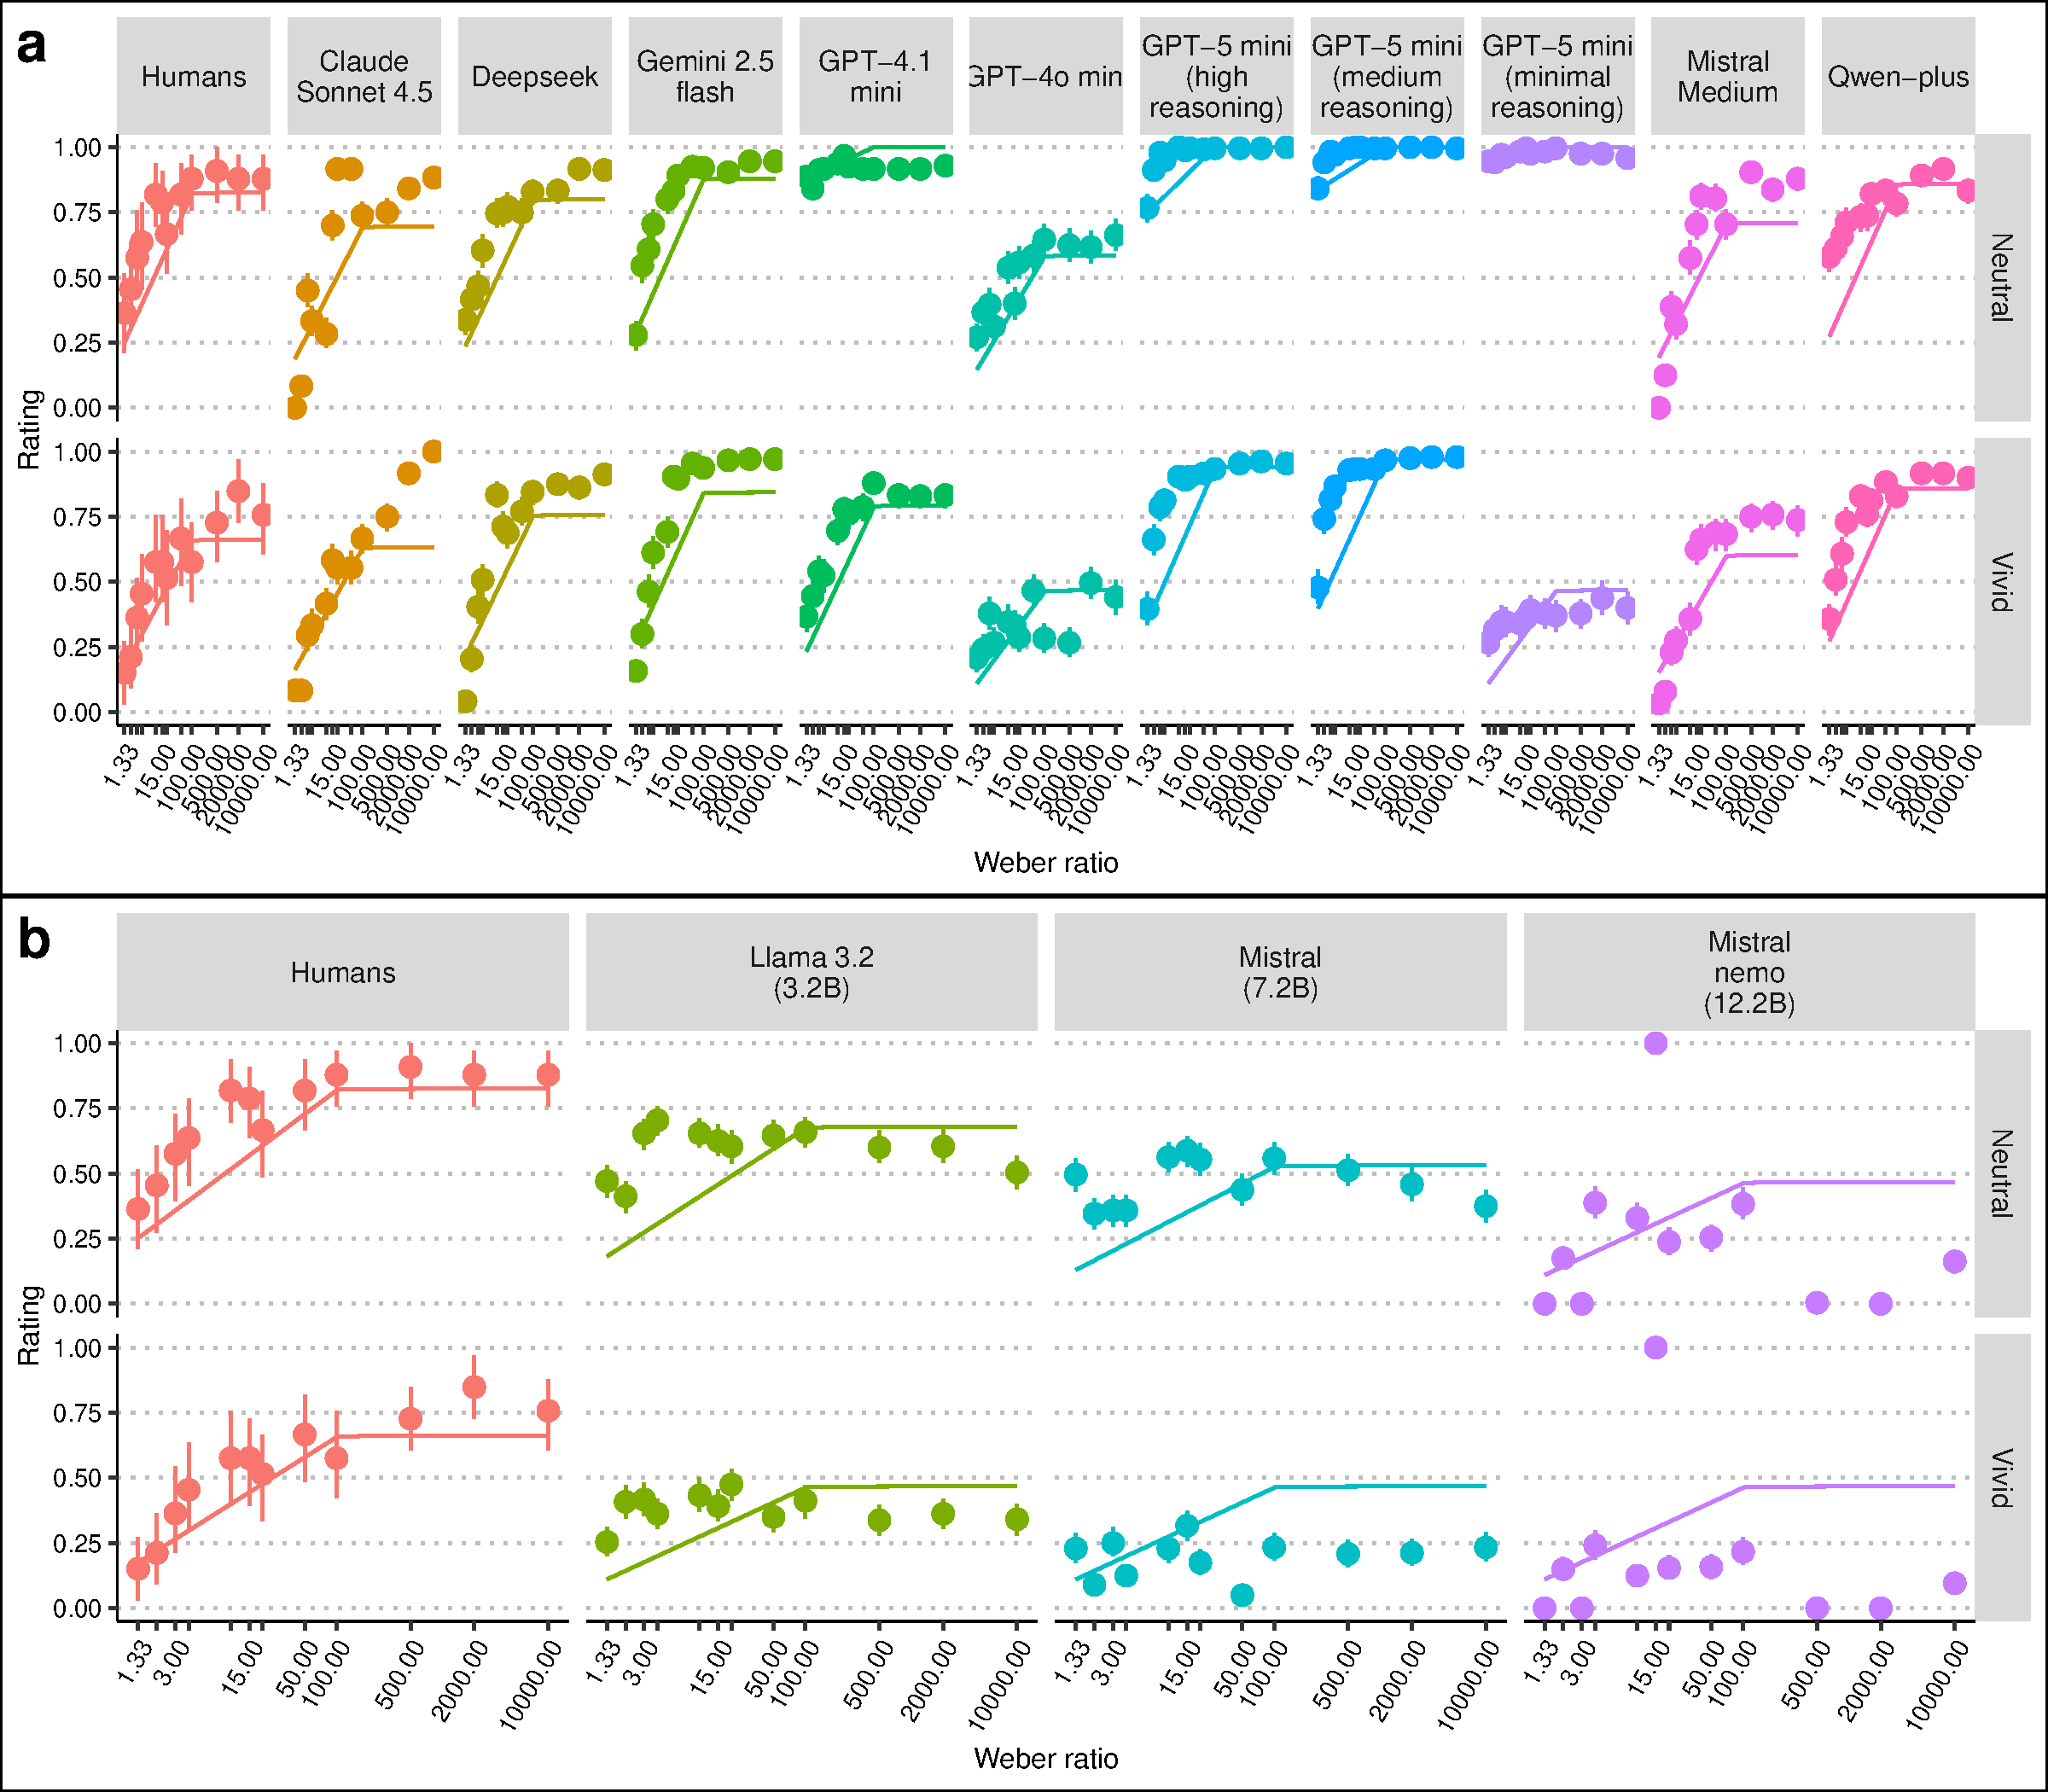
\includegraphics[width=\textwidth,keepaspectratio]{moral_numbers_LLMs_files/figure-latex/plot-llm-results-exp11-ratio-bin-1} 

}

\caption{Acceptability of sacrificial decisions as a function of \emph{beneficiary:victim} Weber ratio in Experiment 6 Data show binarized responses for neutral (top) and vivid (bottom) portrayals of the victims' deaths. Points represent mean acceptability with 95\% confidence intervals. Curves show psychophysical model fits. (a) Frontier models. (b) Cloud models.}\label{fig:plot-llm-results-exp11-ratio-bin}
\end{figure}

\begin{longtable}[t]{llrrrr}
\caption{\label{tab:print-fits-exp11}Psychophysical model parameter estimates for Experiment 6. The $w$ parameter reflects precision in the representations of the numbers of victims and beneficiaries. Higher values indicate greater uncertainty; values greater than 2 indicate the model hit the upper bound of the estimation procedure. The $\alpha$ parameter reflects the attentional weight of the victims. Empty cells indicate convergence failure. Most models showed higher $\alpha$ values in the vivid than neutral condition.}\\
\toprule
\multicolumn{2}{c}{\textbf{ }} & \multicolumn{2}{c}{\textbf{$w$}} & \multicolumn{2}{c}{\textbf{$\alpha$}} \\
\cmidrule(l{3pt}r{3pt}){3-4} \cmidrule(l{3pt}r{3pt}){5-6}
\textbf{Model} & \textbf{Condition} & \textbf{\textit{M}} & \textbf{\textit{SE}} & \textbf{\textit{M}} & \textbf{\textit{SE}}\\
\midrule
\endfirsthead
\caption[]{\label{tab:print-fits-exp11}Psychophysical model parameter estimates for Experiment 6. The $w$ parameter reflects precision in the representations of the numbers of victims and beneficiaries. Higher values indicate greater uncertainty; values greater than 2 indicate the model hit the upper bound of the estimation procedure. The $\alpha$ parameter reflects the attentional weight of the victims. Empty cells indicate convergence failure. Most models showed higher $\alpha$ values in the vivid than neutral condition. \textit{(continued)}}\\
\toprule
\textbf{Model} & \textbf{Condition} & \textbf{\textit{M}} & \textbf{\textit{SE}} & \textbf{\textit{M}} & \textbf{\textit{SE}}\\
\midrule
\endhead

\endfoot
\bottomrule
\endlastfoot
\addlinespace[0.3em]
\multicolumn{6}{l}{\textbf{Humans}}\\
\cellcolor{gray!10}{\hspace{1em}Humans} & \cellcolor{gray!10}{Neutral} & \cellcolor{gray!10}{0.820} & \cellcolor{gray!10}{0.056} & \cellcolor{gray!10}{1.03} & \cellcolor{gray!10}{0.094}\\
\hspace{1em}Humans & Vivid & 1.154 & 0.090 & 1.32 & 0.141\\
\addlinespace[0.3em]
\multicolumn{6}{l}{\textbf{Frontier models}}\\
\cellcolor{gray!10}{\hspace{1em}Claude Sonnet 4.5} & \cellcolor{gray!10}{Neutral} & \cellcolor{gray!10}{0.943} & \cellcolor{gray!10}{0.130} & \cellcolor{gray!10}{1.88} & \cellcolor{gray!10}{0.300}\\
\hspace{1em}Claude Sonnet 4.5 & Vivid & 1.114 & 0.137 & 1.95 & 0.310\\
\cellcolor{gray!10}{\hspace{1em}Deepseek} & \cellcolor{gray!10}{Neutral} & \cellcolor{gray!10}{0.886} & \cellcolor{gray!10}{0.061} & \cellcolor{gray!10}{1.00} & \cellcolor{gray!10}{0.102}\\
\hspace{1em}Deepseek & Vivid & 0.829 & 0.049 & 1.68 & 0.114\\
\cellcolor{gray!10}{\hspace{1em}Gemini 2.5 flash} & \cellcolor{gray!10}{Neutral} & \cellcolor{gray!10}{0.695} & \cellcolor{gray!10}{0.034} & \cellcolor{gray!10}{1.06} & \cellcolor{gray!10}{0.055}\\
\hspace{1em}Gemini 2.5 flash & Vivid & 0.717 & 0.070 & 1.31 & 0.108\\
\cellcolor{gray!10}{\hspace{1em}GPT-4.1 mini} & \cellcolor{gray!10}{Neutral} & \cellcolor{gray!10}{0.485} & \cellcolor{gray!10}{0.127} & \cellcolor{gray!10}{1.00} & \cellcolor{gray!10}{0.178}\\
\hspace{1em}GPT-4.1 mini & Vivid & 0.907 & 0.056 & 1.00 & 0.094\\
\cellcolor{gray!10}{\hspace{1em}GPT-4o mini} & \cellcolor{gray!10}{Neutral} & \cellcolor{gray!10}{1.503} & \cellcolor{gray!10}{0.113} & \cellcolor{gray!10}{1.00} & \cellcolor{gray!10}{0.157}\\
\hspace{1em}GPT-4o mini & Vivid & 2.000 & 0.228 & 1.00 & 0.264\\
\cellcolor{gray!10}{\hspace{1em}GPT-5 mini (high reasoning)} & \cellcolor{gray!10}{Neutral} & \cellcolor{gray!10}{0.211} & \cellcolor{gray!10}{0.072} & \cellcolor{gray!10}{1.00} & \cellcolor{gray!10}{0.106}\\
\hspace{1em}GPT-5 mini (high reasoning) & Vivid & 0.584 & 0.018 & 1.00 & 0.028\\
\cellcolor{gray!10}{\hspace{1em}GPT-5 mini (medium reasoning)} & \cellcolor{gray!10}{Neutral} & \cellcolor{gray!10}{0.162} & \cellcolor{gray!10}{0.144} & \cellcolor{gray!10}{1.00} & \cellcolor{gray!10}{0.266}\\
\hspace{1em}GPT-5 mini (medium reasoning) & Vivid & 0.511 & 0.028 & 1.00 & 0.040\\
\cellcolor{gray!10}{\hspace{1em}GPT-5 mini (minimal reasoning)} & \cellcolor{gray!10}{Neutral} & \cellcolor{gray!10}{0.112} & \cellcolor{gray!10}{6.932} & \cellcolor{gray!10}{1.00} & \cellcolor{gray!10}{18.427}\\
\hspace{1em}GPT-5 mini (minimal reasoning) & Vivid & 2.000 & 0.169 & 1.00 & 0.196\\
\cellcolor{gray!10}{\hspace{1em}Mistral Medium} & \cellcolor{gray!10}{Neutral} & \cellcolor{gray!10}{0.910} & \cellcolor{gray!10}{0.071} & \cellcolor{gray!10}{1.87} & \cellcolor{gray!10}{0.164}\\
\hspace{1em}Mistral Medium & Vivid & 1.139 & 0.082 & 2.38 & 0.266\\
\cellcolor{gray!10}{\hspace{1em}Qwen-plus} & \cellcolor{gray!10}{Neutral} & \cellcolor{gray!10}{0.798} & \cellcolor{gray!10}{0.080} & \cellcolor{gray!10}{1.00} & \cellcolor{gray!10}{0.136}\\
\hspace{1em}Qwen-plus & Vivid & 0.760 & 0.037 & 1.00 & 0.062\\
\addlinespace[0.3em]
\multicolumn{6}{l}{\textbf{Local models}}\\
\cellcolor{gray!10}{\hspace{1em}Llama 3.2 (3.2B)} & \cellcolor{gray!10}{Neutral} & \cellcolor{gray!10}{1.190} & \cellcolor{gray!10}{0.129} & \cellcolor{gray!10}{1.00} & \cellcolor{gray!10}{0.202}\\
\hspace{1em}Llama 3.2 (3.2B) & Vivid & 2.000 & 0.212 & 1.00 & 0.245\\
\cellcolor{gray!10}{\hspace{1em}Mistral (7.2B)} & \cellcolor{gray!10}{Neutral} & \cellcolor{gray!10}{1.795} & \cellcolor{gray!10}{0.231} & \cellcolor{gray!10}{1.00} & \cellcolor{gray!10}{0.288}\\
\hspace{1em}Mistral (7.2B) & Vivid & 2.000 & 0.479 & 1.29 & 0.575\\
\cellcolor{gray!10}{\hspace{1em}Mistral nemo (12.2B)} & \cellcolor{gray!10}{Neutral} & \cellcolor{gray!10}{2.000} & \cellcolor{gray!10}{0.641} & \cellcolor{gray!10}{1.57} & \cellcolor{gray!10}{1.066}\\
\hspace{1em}Mistral nemo (12.2B) & Vivid & 2.000 & 0.714 & 1.97 & 1.237\\*
\end{longtable}

\clearpage

\paragraph{Local models}\label{local-models-2}

\begin{figure}

{\centering 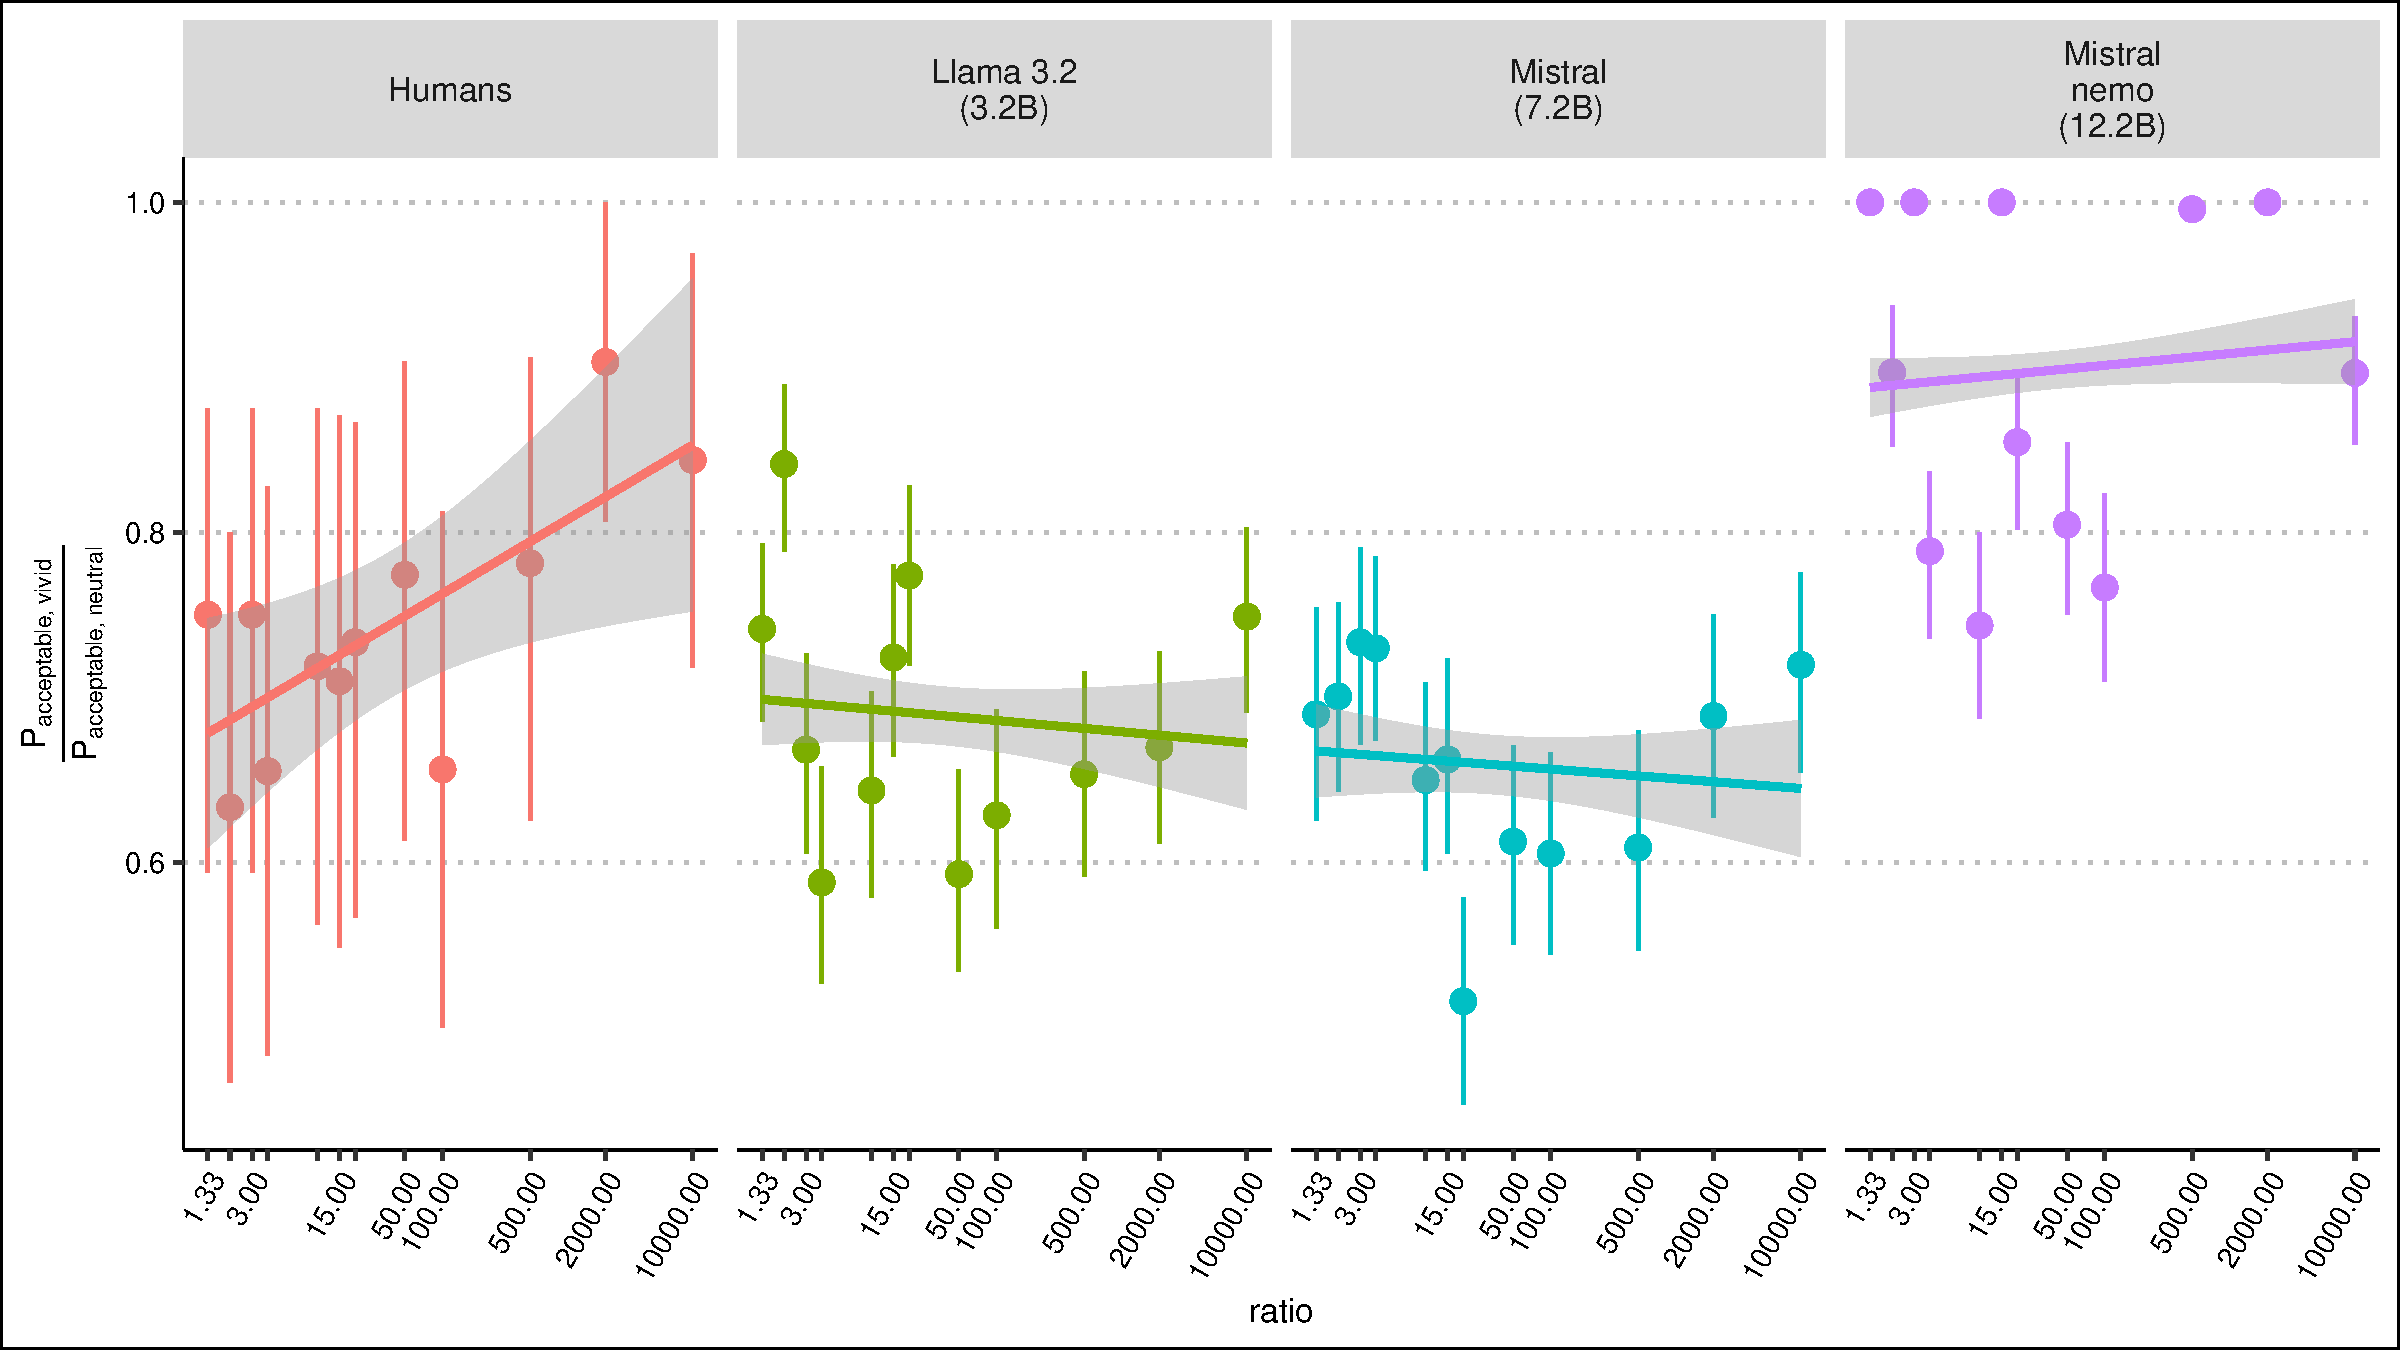
\includegraphics[width=\textwidth,keepaspectratio]{moral_numbers_LLMs_files/figure-latex/exp11-models-relative-risk-plot-local-1} 

}

\caption{Risk ratio of acceptability judgements as a function of \emph{beneficiary:victim} Weber ratio in Experiment 6 for local models. The risk ratio compares acceptability rates when victims' deaths were portrayed vividly or in the same neutral language as the beneficiaries' deaths, $\mathrm{RR}= \frac{P_{\text{acceptable, vivid}}}{P_{\text{acceptable, neutral}}}$. Points show mean risk ratios with 95\% confidence intervals. Regression lines show the relationship between Weber ratio and risk ratio. In humans, higher Weber ratios are associated with higher risk ratios, indicating that the effect of the salience of the victims' deaths portrayals is reduced for higher \emph{beneficiary:victim} ratios. Local models largely failed to reproduce the human pattern: one model (Mistral 7.2B) showed a negative correlation, while the other two models showed no correlation.}\label{fig:exp11-models-relative-risk-plot-local}
\end{figure}

We performed similar analyses for the local models. While the Mistral (7.2B parameters) showed a negative correlation between the risk ratio and the Weber ratio, the other two models showed no correlation.

We also present the acceptability ratings and model fits in Figure \ref{fig:plot-llm-results-exp11-ratio-bin} and Table \ref{tab:print-fits-exp11}, respectively.

\paragraph{Summary}\label{summary-2}

Overall, these results suggest that the models generally reproduced the correlation between the risk ratio and the Weber ratio, though the quantitative fit is of variable quality.

\subsection{Overall Summary}\label{overall-summary}

The frontier LLMs showed several key similarities to human moral judgment. Most models demonstrated sensitivity to \emph{beneficiary:victim} Weber ratios, greater acceptance of sacrifices in economic versus moral decisions, and a decreasing effect of victim salience at higher Weber ratios. However, the quantitative fit to the psychophysical model varied considerably across models, and some models failed to show expected patterns.

These similarities appeared to depend on model size and presumably on massive amounts of training data (or on differences in alignment processes), as the smaller local models largely failed to reproduce human behavior. Local models showed no discernible sensitivity to Weber ratios in Experiment 2 and exhibited inconsistent patterns across other experiments.

However, all models behaved qualitatively differently from humans in Experiment 3. They were more sensitive to both harm and utility than humans, especially in moral situations. In particular, no model showed a preference for Weber ratios over both harm and utility in moral situations.

\bibliography{/Users/endress/ansgar.bib}

\end{document}
